% Author : Ali Snedden
% Date   : 10-feb-2022
% License: MIT (for my content), images licensed appropriately
% Purpose: 
%   This is my nerd hour presentation for the Batelle Center for Mathematical Medicine
% 







\documentclass{beamer}
\usetheme{Copenhagen}
%\usecolortheme{seahorse}
% See http://www.hartwork.org/beamer-theme-matrix/ for more themes and colors

\usepackage{times}  % fonts are up to you
\usepackage{graphics}
\usepackage{amsmath}
\usepackage{media9}
\usepackage{hyperref}

\usepackage{tikz}
\usetikzlibrary{fit}

%Bibliography stuff
%\usepackage[style=authoryear]{biblatex}
\bibliography{/Users/ali/Library/texmf/bibtex/bib/references}
%\bibliographystyle{apj}

\setbeamertemplate{bibliography item}[text]
%\usepackage[backend=bibtex, style=authoryear]{biblatex}
%\addbibresource{/Users/ali/Library/texmf/bibtex/bib/references.bib}
\newcommand{\customcite}[1]{\citeauthor{#1}, \citeyear{#1}}
% https://tex.stackexchange.com/a/61016/84495
\newcommand{\chref}[3][blue]{\href{#2}{\color{#1}{#3}}}%


\newcommand\smallFont{\fontsize{8}{7.2}\selectfont}   %Change font size.
\newcommand\mCite[1]{[\cite{#1}, \citetitle{#1}]}  %Prints name and title
\newcommand\FrameText[1]{
\begin{textblock*}{\paperwidth}(0pt,\textheight)
    \vspace{1.0cm}
    \raggedleft \smallFont #1
\end{textblock*}}

%Get rid of ugly copenhagen default symbol for enumerate
\setbeamertemplate{enumerate items}[default]   

%Increase default separation size between items in itemize and enumerate 
\tikzset{type1/.style={rectangle, rounded corners, minimum width=3cm, minimum height=0.1cm,text centered, draw=black, fill=blue!10, text width=2cm},
        type2/.style={rectangle, rounded corners, minimum width=3cm, minimum height=0.1cm, text centered, draw=black, fill=blue!10, text width=5cm},
        info/.style = {rectangle, rounded corners, minimum width=2.5cm, minimum height=0.1cm, text centered, draw=black, 
            fill=blue!30, text width=2.5cm},
        org/.style={rectangle, rounded corners, minimum width=2cm, minimum height=0.1cm, text centered, draw=black, 
            fill=blue!30, text width=3cm},
        decision/.style = {square, minimum width=1cm, minimum height=0.1cm, text centered, 
            draw=black, fill=green!30, text width=4cm},
        arrow/.style = {thick,->,>=stealth},
    }
    
    
    
   

%%%%%%%%%%%%%%% BIBLIOGRAPHY COMMANDS %%%%%%%%%%%%%%%
\newcommand{\apj}{ApJ.}
\newcommand{\apjs}{ApJS}
\newcommand{\apjl}{ApJL}
\newcommand{\pasp}{Publications of the Astronomical Society of the Pacific}
\newcommand{\pasj}{Publ. of the Astron. Soc. of Japan}
\newcommand{\prc}{Phys. Rev. C}
\newcommand{\prd}{Phys. Rev. D}
\newcommand{\nat}{Nature}
\newcommand{\mnras}{Mon. Not. R. Astron. Soc.}
\newcommand{\na}{New Astronomy}
\newcommand{\aap}{Astronomy and Astrophysics}
\newcommand{\araa}{Annu. Rev. Astron. Astrophys}
\newcommand{\aj}{Astronomical Journal}
\newcommand{\pasa}{Pub. of the Astron. Soc. of Australia}
\newcommand{\nar}{New Astronomy Reviews}


%%%%%%%%%%%%%%% OTHER COMMANDS %%%%%%%%%%%%%%%%%
\newcommand{\subitem}{\item[$-$]}

% these will be used later in the title page
\title{Is anyone out there?}
\author{Ali Snedden
}
\date{February 10, 2022}
%\subtitle{stuff}

% note: do NOT include a \maketitle line; also note that this title
% material goes BEFORE the \begin{document}

% Recurring Outline
\AtBeginSection[]  % "Beamer, do the following at the start of every section"
{
\begin{frame}<beamer> 
\frametitle{Outline} % make a frame titled "Outline"
\tableofcontents[currentsection]  % show TOC and highlight current section
\end{frame}
}

\begin{document}

% this prints title, author etc. info from above
\begin{frame}
\titlepage
\end{frame}



%%%%%%%%%%%%%%%%%%%%%%%%%%%%%%%%%%%%%%%%%%%%%%%%%%%
%%%%%%%%%%%%%% History : Pre-Modern %%%%%%%%%%%%%%%
%%%%%%%%%%%%%%%%%%%%%%%%%%%%%%%%%%%%%%%%%%%%%%%%%%%
%\section{History : Pre-Modern (pre-$20^{th}$ century)}
\section{History}
%%% % TO DO Cite tippler here, add pictures
\begin{frame}
\frametitle{Antiquity}
\begin{picture}(320,250) 
\visible<1-2>{\put(200, 100){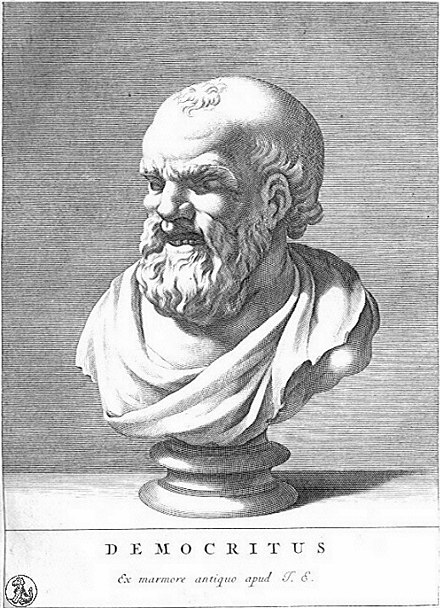
\includegraphics[height=1.5in]{images/democritus-PD.jpg}}}
\visible<3>{\put(200, 100){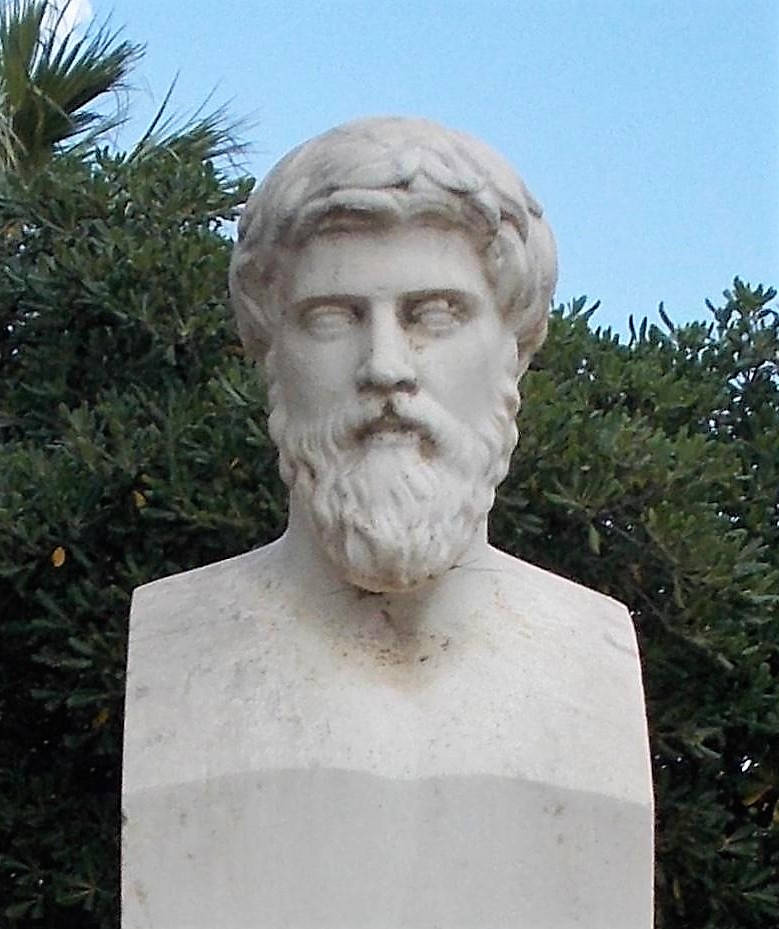
\includegraphics[height=1.5in]{images/plutarch-cc-by-sa4.jpg}}}
\put(-20, 220){\begin{minipage}[t]{0.6 \linewidth}
{
    ``Believers" in life on other planets
        \begin{itemize}
            \item Democritus (atomic theory of the universe, geometry)
            %\put(150, 200){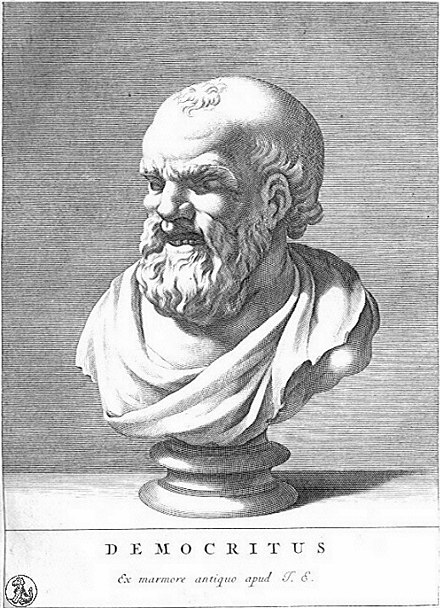
\includegraphics[height=0.75in]{images/democritus-PD.jpg}}
                %{\scriptsize{Democritus (atomic theory of universe}}
            \pause
            \item Metrodorus of Chios 
                \begin{enumerate}
                    \item[--] ``It seems absurd, that in a large field only one stalk
                                should grow, and that in an infinite space only one world
                                exist."
                \end{enumerate}
            \pause
            % Contmporary of Nero of fiddle fame
            \item Plutarch (historian, contemporary of Nero)
        \end{itemize}
}
\end{minipage}}
\end{picture}
\end{frame}

\begin{frame}
\frametitle{Antiquity}
\begin{picture}(320,250) 
\visible<1>{\put(200, 100){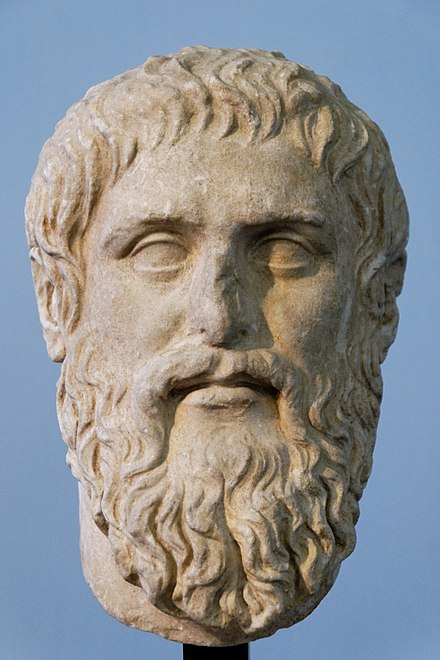
\includegraphics[height=1.5in]{images/plato-PD.jpg}}}
\visible<2->{\put(200, 100){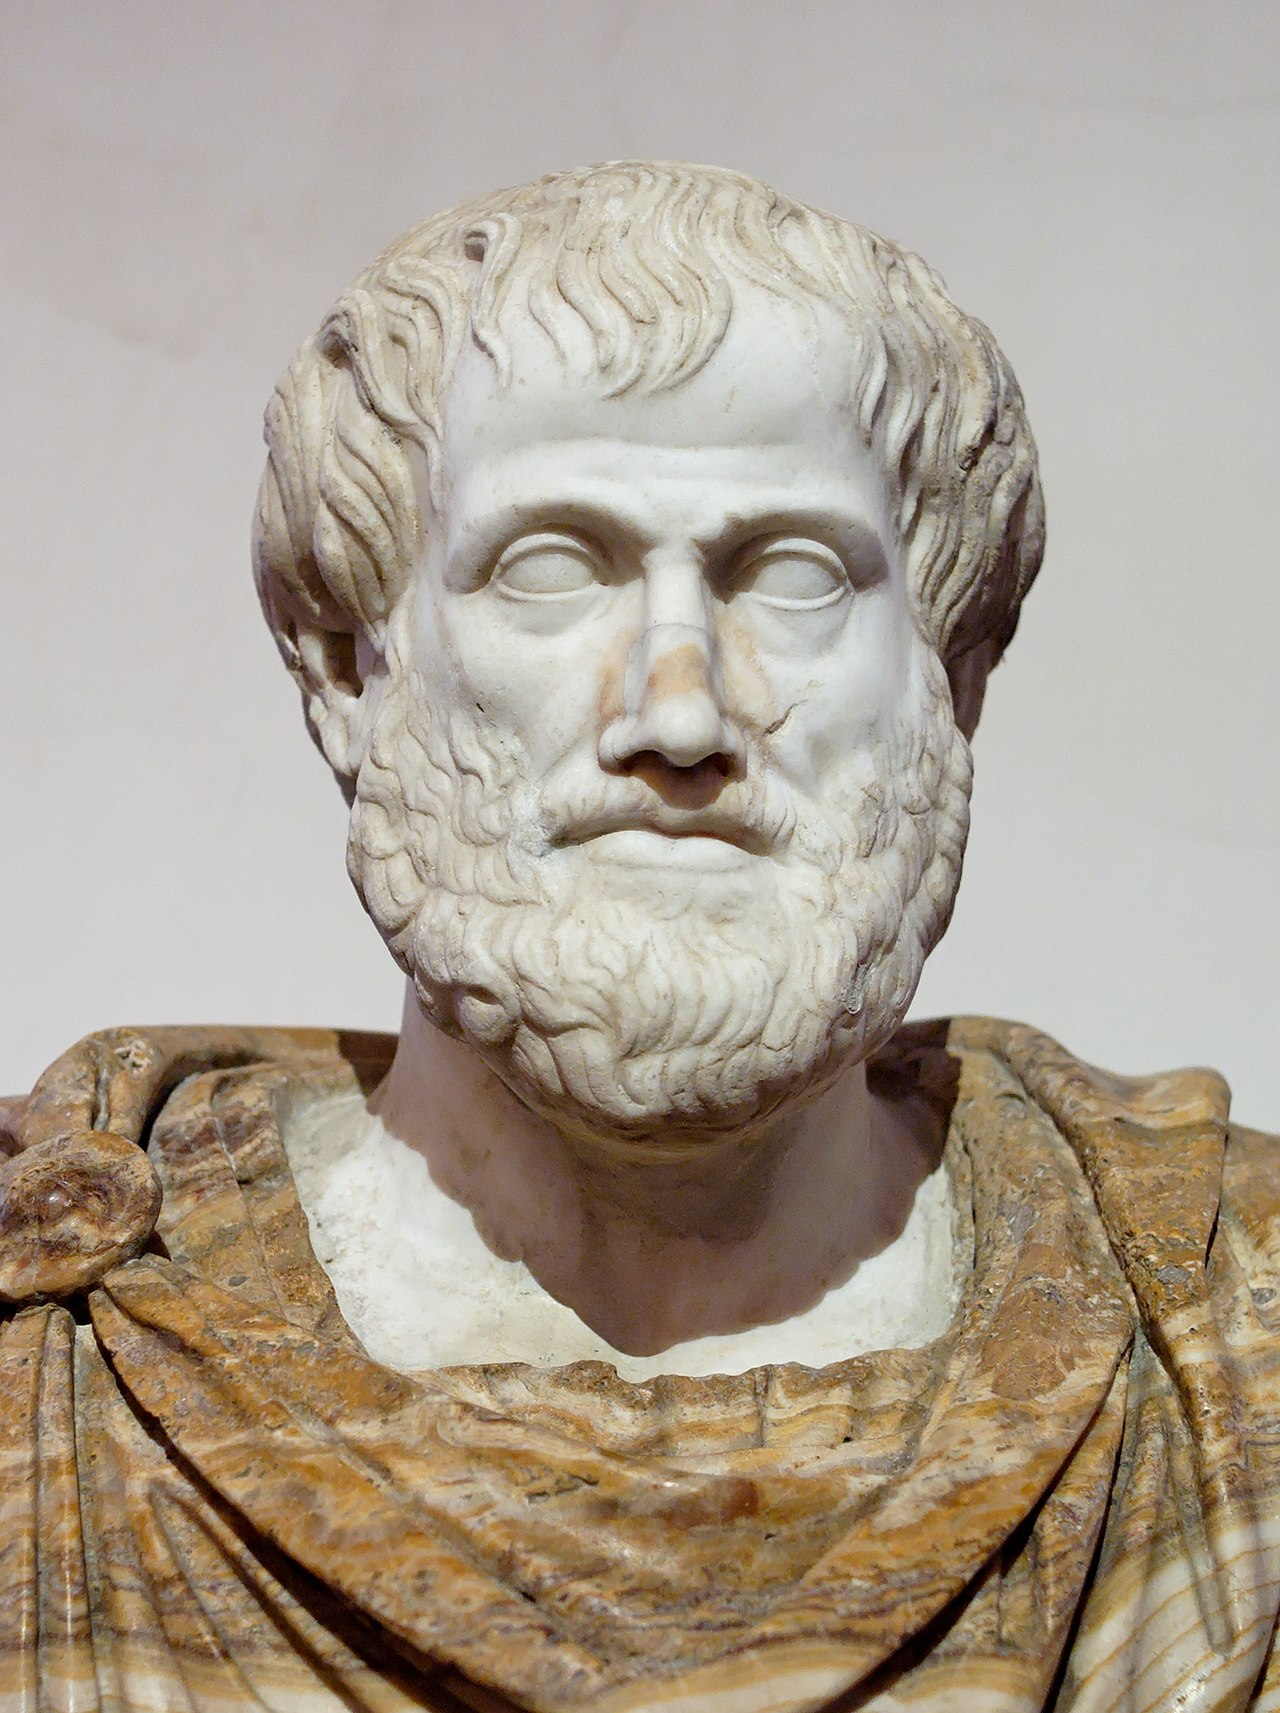
\includegraphics[height=1.5in]{images/aristotle-PD.jpg}}}
\put(-20, 220){\begin{minipage}[t]{0.6 \linewidth}
{
    ``Non-believers" in life on other planets
        \begin{itemize}
            \item Plato (philosopher)
            \pause
            \item Aristotle (philosopher)
                \begin{enumerate}
                    \item[--] Universe of Aristotle is finite, with only one inhabited planet
                \end{enumerate}
        \end{itemize}
}
\end{minipage}}
\end{picture}
\end{frame}

\begin{frame}
\frametitle{Christian Era}
\begin{picture}(320,250) 
\visible<1>{\put(230, 100){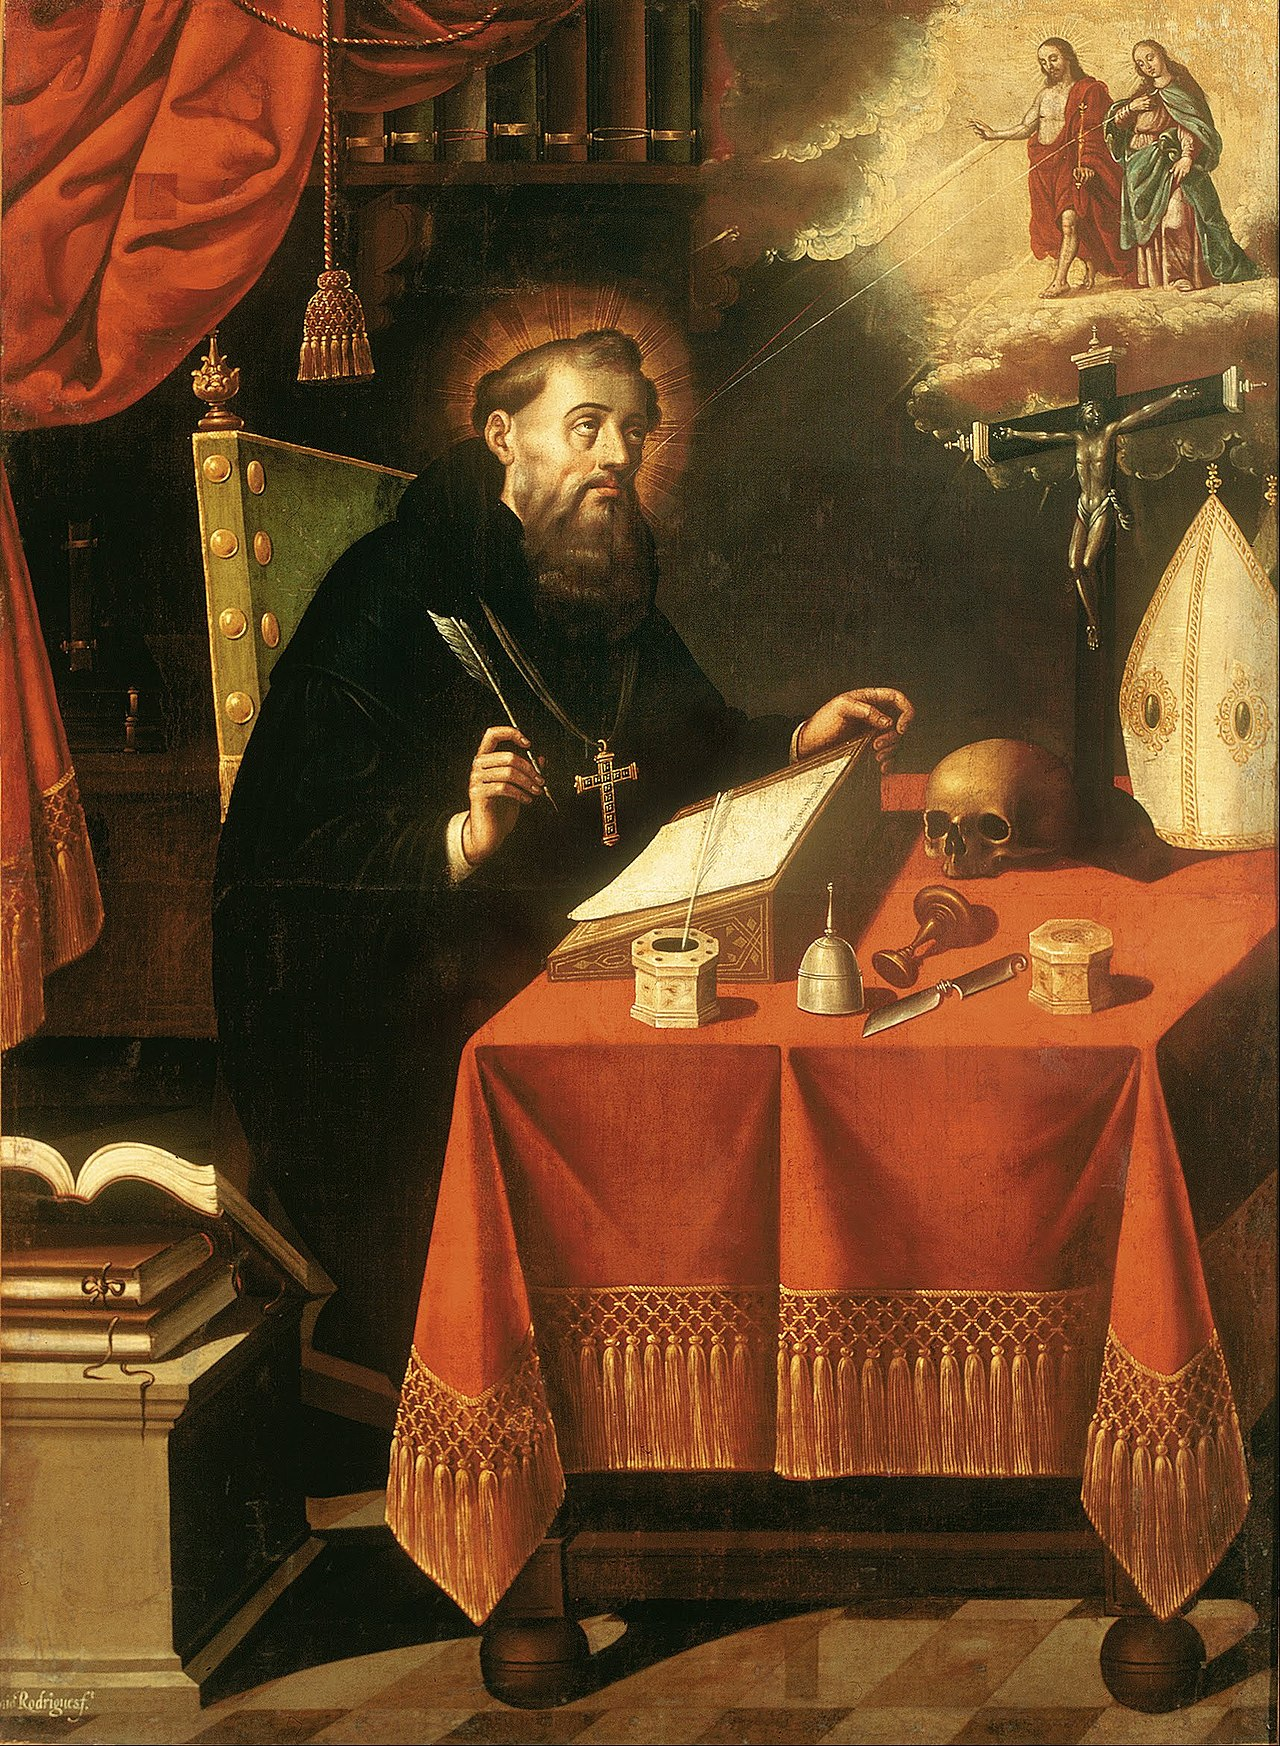
\includegraphics[height=1.5in]{images/st-augustine-PD.jpg}}}
\visible<2>{\put(230, 100){
\includegraphics[height=1.5in]{images/albertus-magnus-PD.jpg}}}
\visible<3>{\put(230, 100){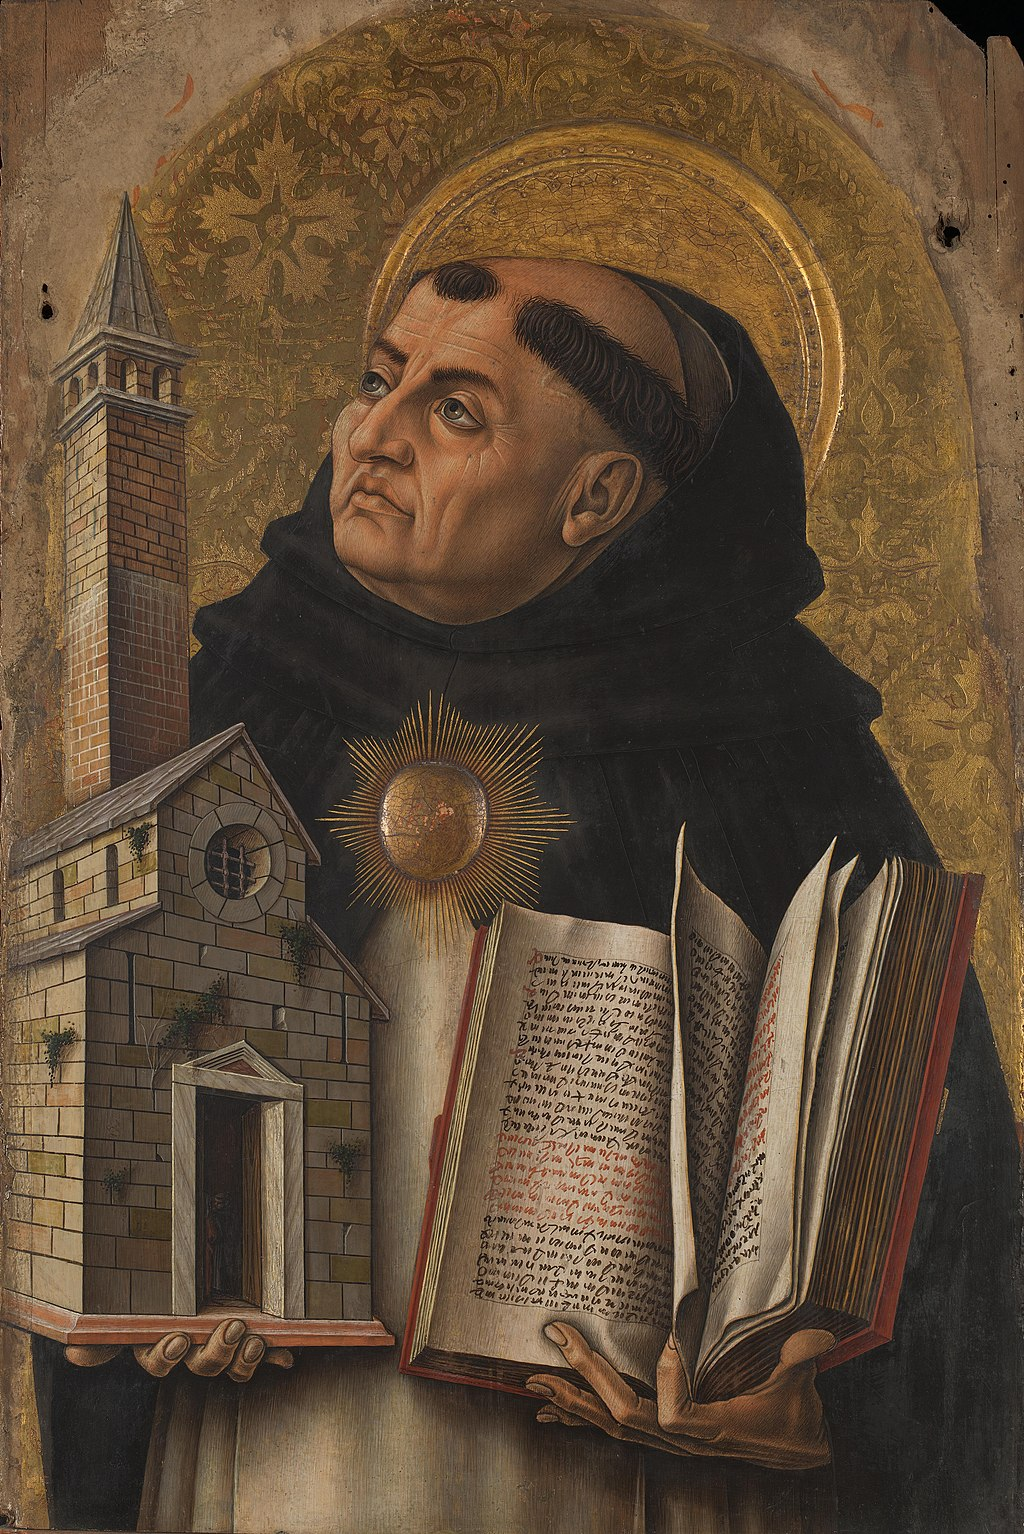
\includegraphics[height=1.5in]{images/thomas-aquinas-PD.jpg}}}
\put(-20, 240){\begin{minipage}[t]{0.8 \linewidth}
{
    ``Non-believers" 
        \begin{itemize}
            \item St. Augustine (Theologian)
                \begin{enumerate}
                    \item If other intelligent beigns similar to man existed, then they'd 
                              also require a savior, which would contradict the uniqueness of
                              Christ (I Peter 3:18)
                \end{enumerate}
            % Commented on Aristotle, Discovered Arsenic - against b/c of uniqueness of incarnations
            \pause
            \item St. Albertus Magnus (Friar, Philosopher, Scientist)
                \begin{enumerate}
                    \item ``Do there exist many worlds or is there but a single world?
                              This is one of the most noble and exalted questions in the
                              study of Nature"
                \end{enumerate}
            % Influential Philosopher
            \pause
            \item St. Thomas Aquinas (Philosopher, Theologian)
                \begin{enumerate}
                    \item If God made similar worlds, they would be in vain and 
                               inconsistent with Divine Wisdom.
                \end{enumerate}
        \end{itemize}
}
\end{minipage}}
\end{picture}
\end{frame}


\begin{frame}
\frametitle{Renaissance }
\begin{picture}(320,250) 
%\visible<1>{\put(230, 100){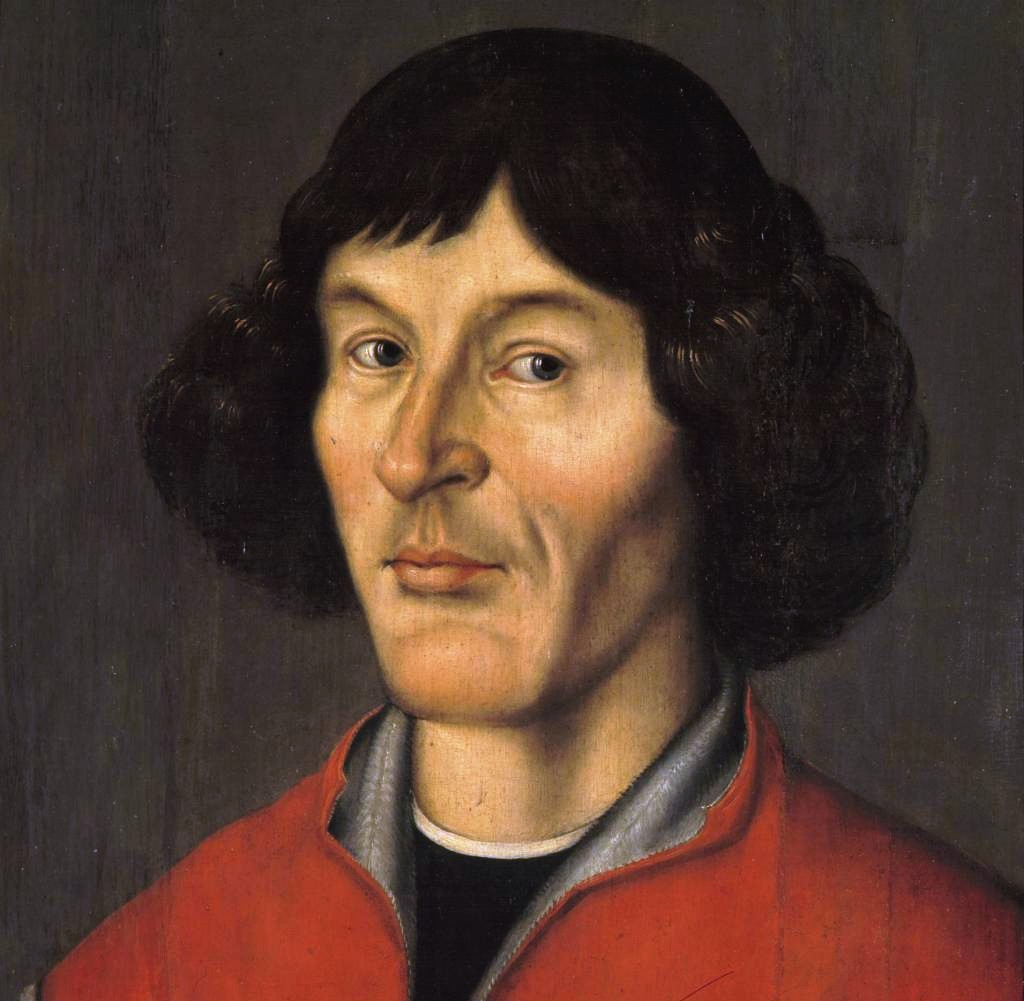
\includegraphics[height=1.5in]{images/nicolaus-copernicus-PD.jpg}}}
\visible<1>{\put(240, 100){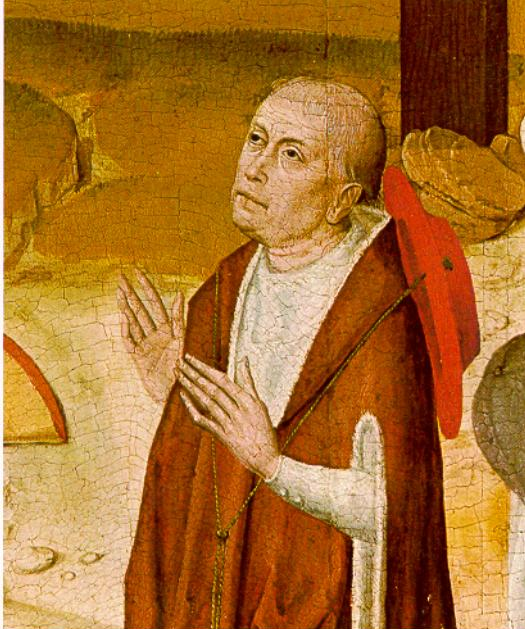
\includegraphics[height=1.5in]{images/nicholas_of_cusa-PD.jpg}}}
\visible<2>{\put(240, 100){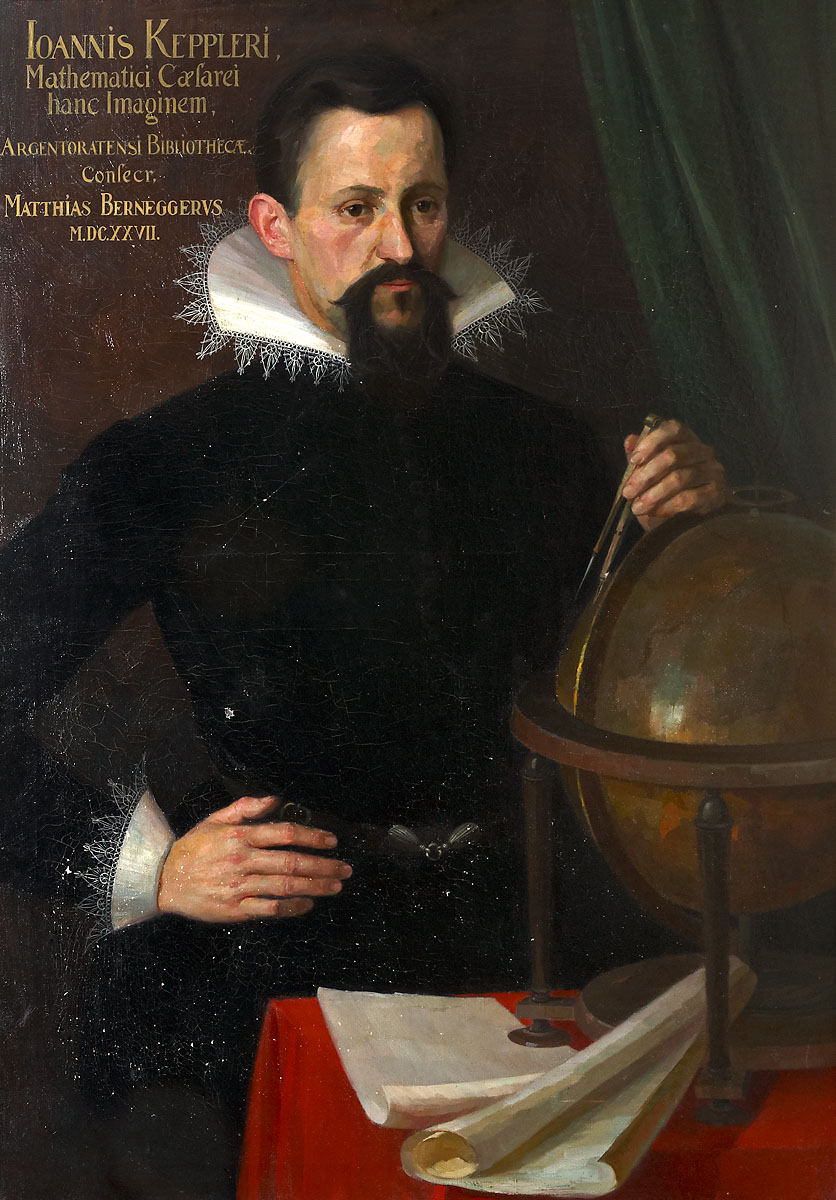
\includegraphics[height=1.5in]{images/jkepler-PD.jpg}}}
\visible<3>{\put(240, 100){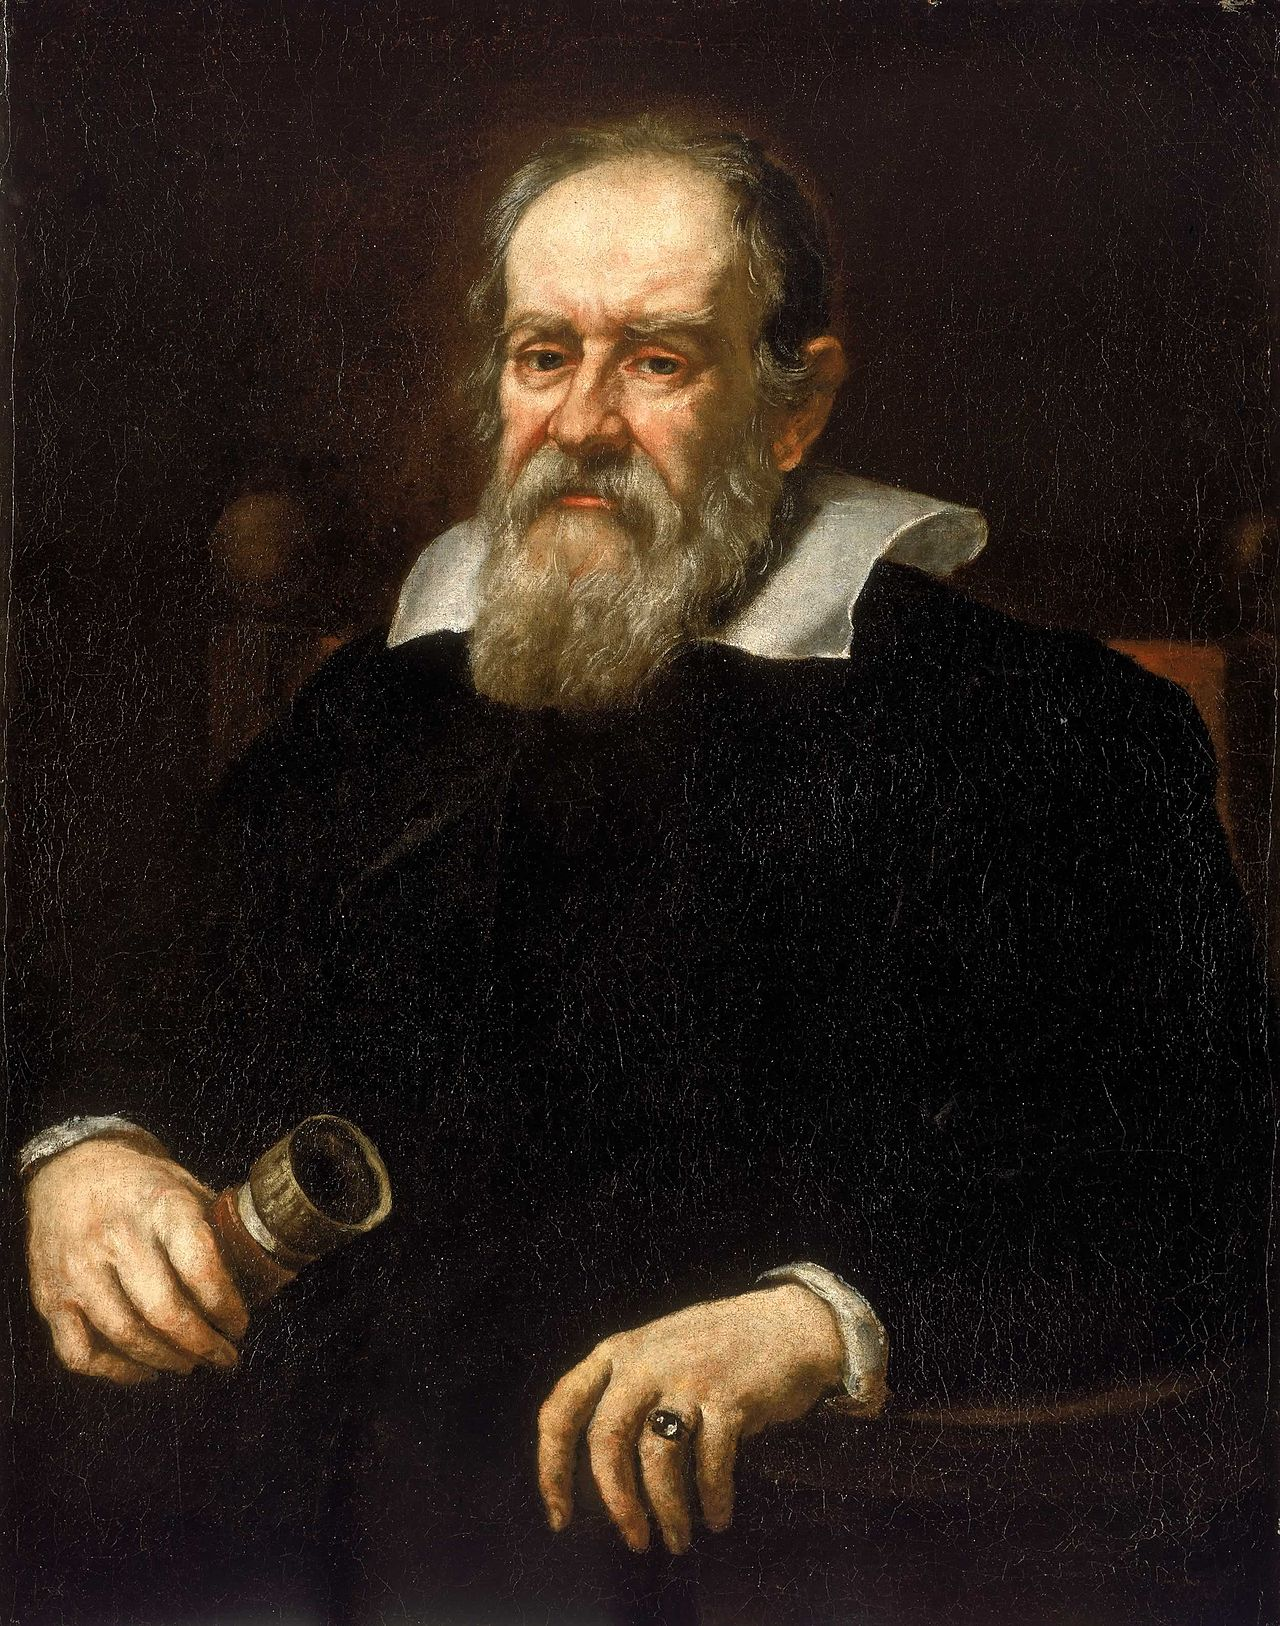
\includegraphics[height=1.5in]{images/galileo-galilei-PD.jpg}}}
\put(-20, 240){\begin{minipage}[t]{0.85 \linewidth}
{
    ``Believers" : 
        \begin{itemize}
            % Open to intelligent life
            %\item Nicholaus Copernicus 
            \item Nicholas of Cusa (astronomer, theologian, cleric)
                \begin{enumerate}
                    \item Believed plurality of worlds around other stars with intelligent beings
                \end{enumerate}
            \pause
            % Maybe life, nothing like humans
        \end{itemize}
    ``Non-believers" : 
        \begin{itemize}
            \item Johannes Kepler
                \begin{enumerate}
                    \item "No moons have yet been seen revolving around [the stars].
                               Hence this will remain an open question until this
                               phenomenon too is detected"
                \end{enumerate}
            \pause
            % Non-believer
            \item Galileo Galilei (telescope, Jupiter's moons)
                \begin{enumerate}
                    \item "... false and damnable the view of those who would put
                               inhabitants on Jupiter, Venus, Saturn and the Moon, meaning
                               by `inhabitants' animals like ours and men in particular"
                \end{enumerate}
        \end{itemize}
}
\end{minipage}}
\end{picture}
\end{frame}


\begin{frame}
\frametitle{Enlightenment}
\begin{picture}(320,250) 
\put(230, 100){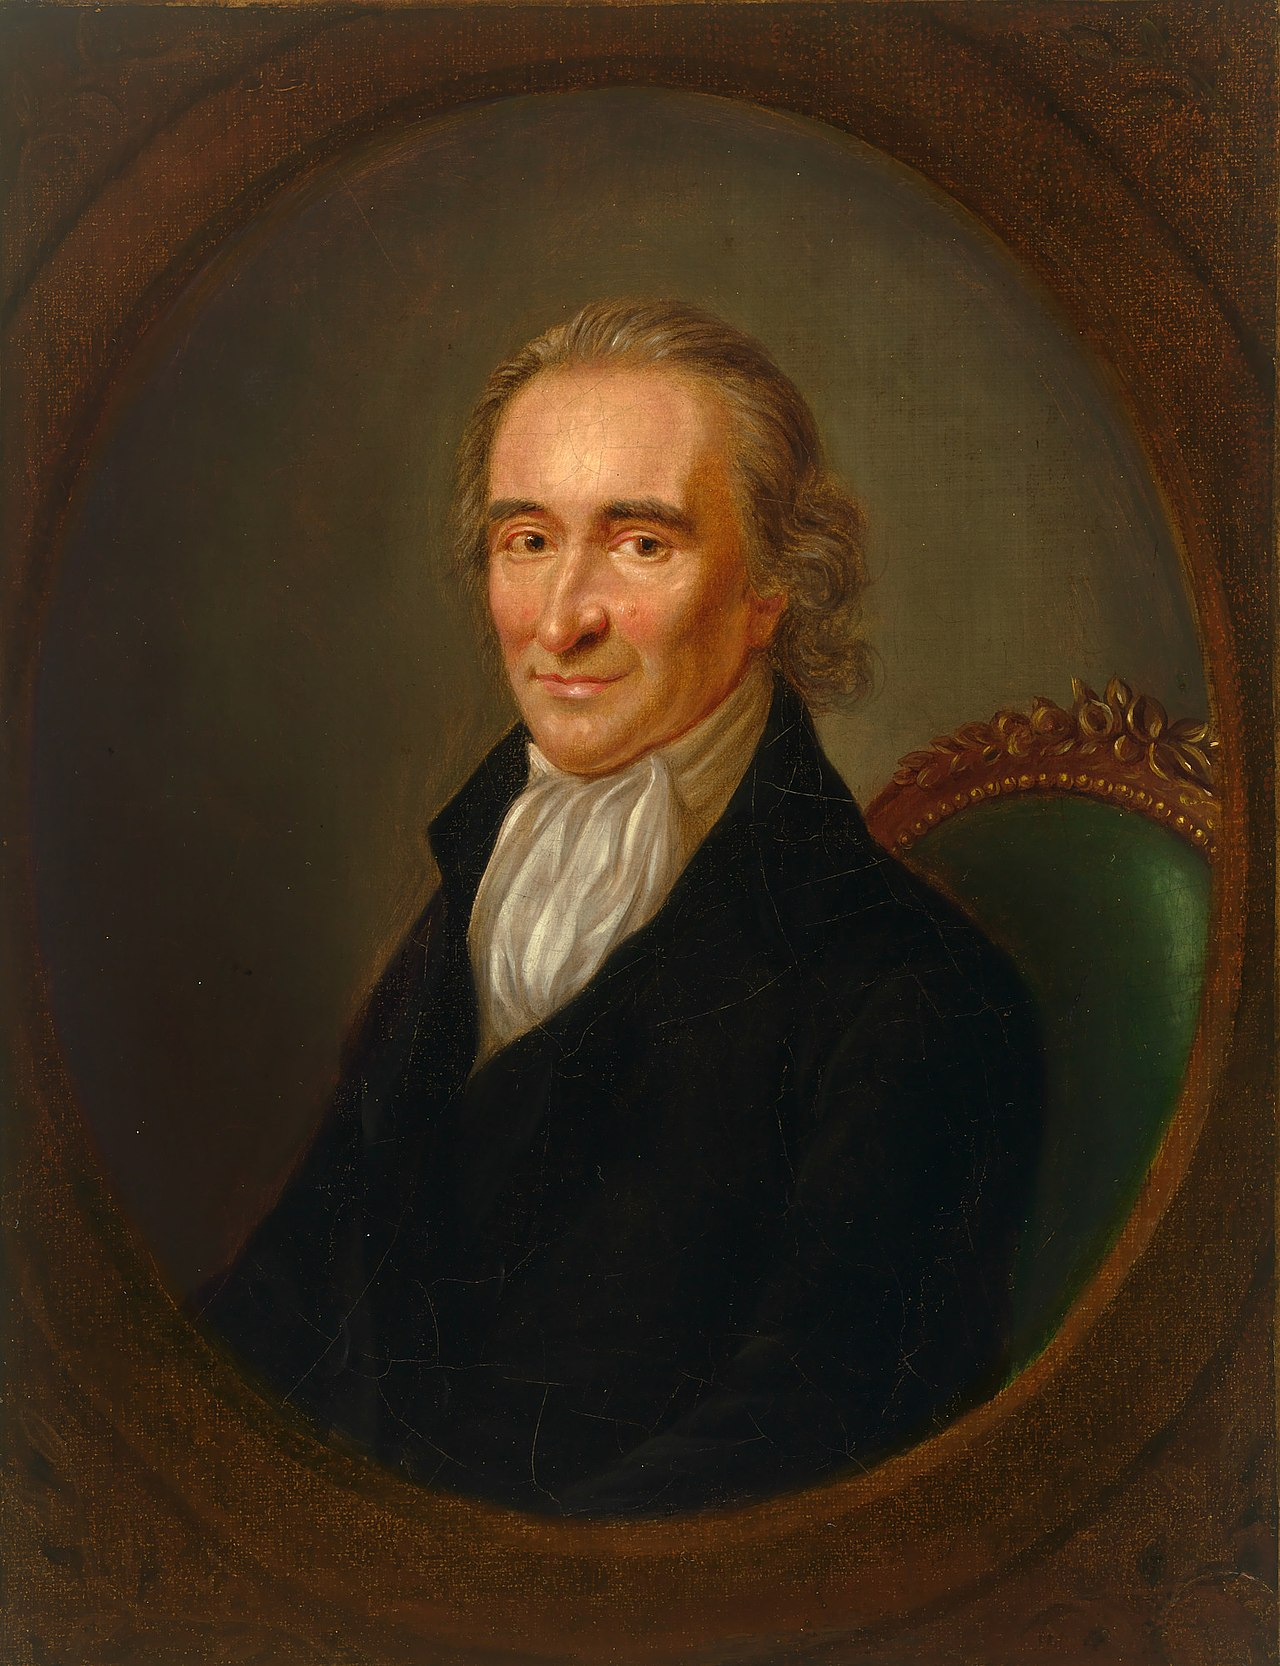
\includegraphics[height=1.5in]{images/thomas-paine-PD.jpg}}
\put(-20, 220){\begin{minipage}[t]{0.8 \linewidth}
{
    ``Believer" 
        \begin{enumerate}
            % Open to intelligent life - clear rejection of uniquenss of incarnations
            \item Thomas Paine (revolutionary, author)
                \begin{itemize}
                    \item[--]
                  From whence then could arise the solitary and strange conceit that the
                  Almighty, who had millions of worlds equally dependent on his protection,
                  should quit the care of all the rest, and come to die in our world,
                  because, they say, one man and one woman had eaten an apple!
                  %And, on
                  %the other hand, are we to suppose that every world in the boundless 
                  %creation had an Eve, an apple, a serpent, and a redeemer?
                  %In this case, the
                  %person who is irreverently called the Son of God, and sometimes God
                  %himself, would have nothing else to do than to travel from world to
                  %world, in an endless succession of death, with scarcely a momentary
                  %interval of life "
                \end{itemize}
        \end{enumerate}
}
\end{minipage}}
\end{picture}
\end{frame}


\begin{frame}
\frametitle{Modern Era}
\begin{picture}(320,250) 
\visible<1>{\put(240, 100){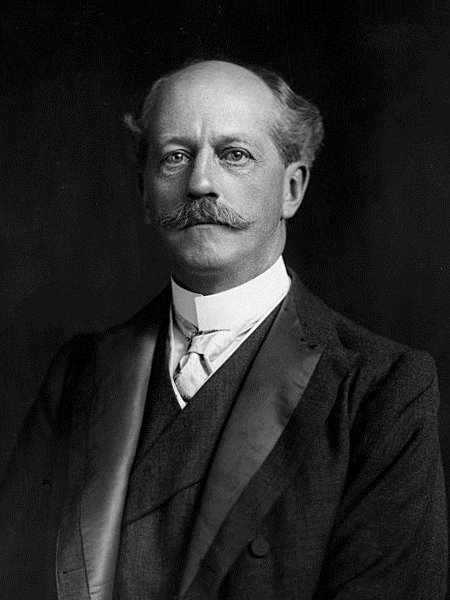
\includegraphics[height=1.5in]{images/lowell-PD.jpg}}}
\visible<2>{\put(240, 100){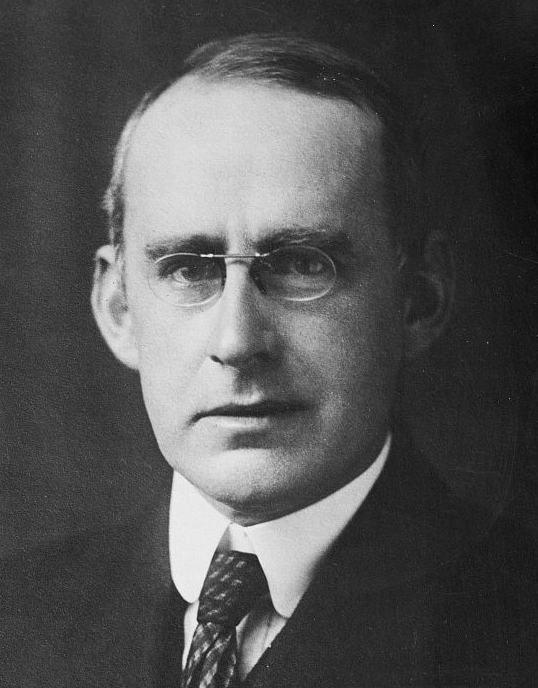
\includegraphics[height=1.5in]{images/eddington-PD.jpg}}}
\visible<3>{\put(240, 100){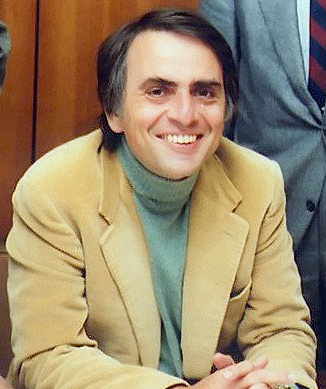
\includegraphics[height=1.5in]{images/sagan-PD.png}}}
\put(-20, 240){\begin{minipage}[t]{0.8 \linewidth}
{
    ``Believer" 
        \begin{itemize}
            % 
            \item Percival Lowell (astronomer, canals on Mars)
                \begin{enumerate}
                  {\small
                    \item Quickly discounted by professional astronomers, but caught on
                              in popular press
                  }
                \end{enumerate}
            \pause
            \item Sir Arthur Eddington (astronomer)
                \begin{enumerate}
                  {\small
                    \item ``I do not think that the whole of the Creation has been staked on
                               one planet where we live; and in the long run we cannot deem 
                               ourselves the only race that has been gifted with the mystery    
                               of consciousness"
                  }
                \end{enumerate}
            \pause
            \item Carl Sagan and Frank Drake (astronomers)
                \begin{enumerate}
                  {\small
                    \item ``...little doubt that civilizations more
                               advanced than the earth's exist elsewhere in the universe.
                               The probabilities involved in locating them  call
                               for a substantial effort." 
                  }
                \end{enumerate}
        \end{itemize}
}
\end{minipage}}
\end{picture}
\end{frame}


\begin{frame}
\frametitle{Popular Culture}
\begin{picture}(320,250) 
\put(50, 150){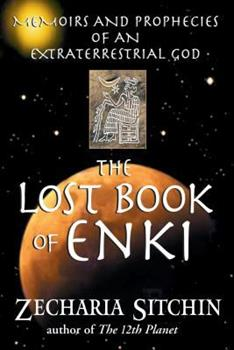
\includegraphics[height=1.25in, width=1.0in]{images/the_lost_book_of_enki-FU.jpg}}
\pause
\put(200, 150){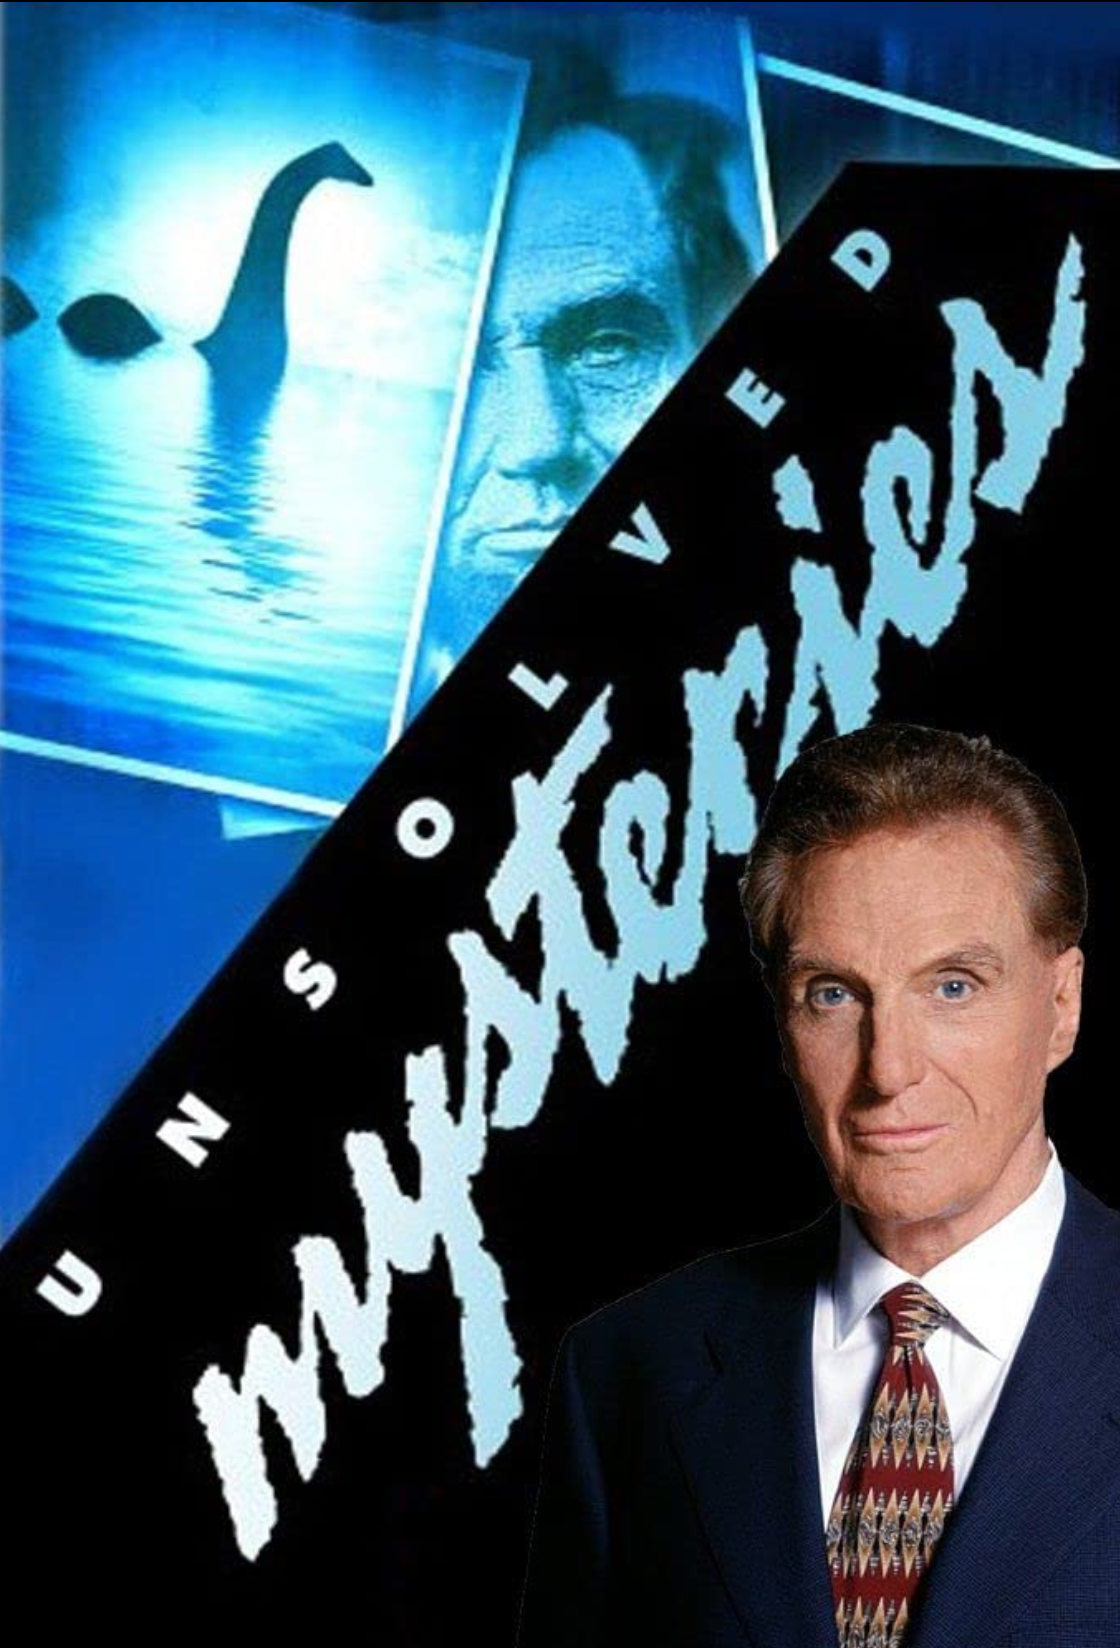
\includegraphics[height=1.25in, width=1.0in]{images/unsolved-mysteries-FU.png}}
\pause
\put(50, 50){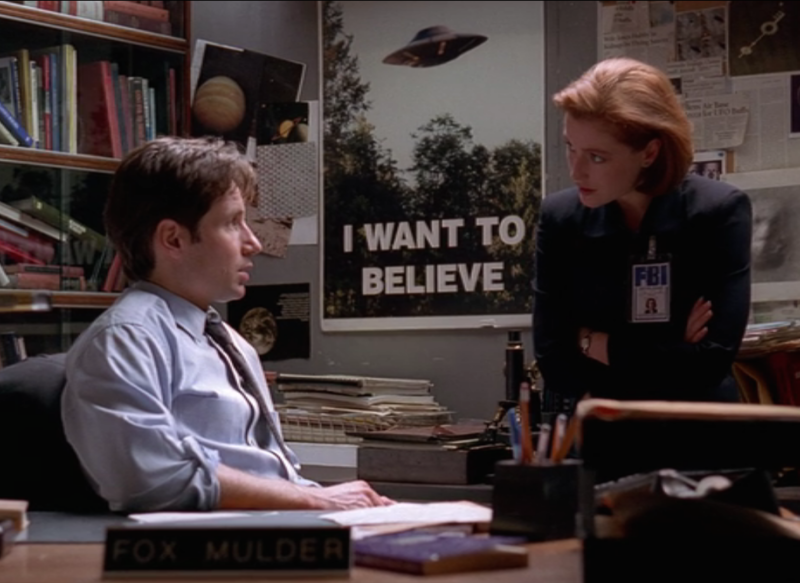
\includegraphics[height=1.25in]{images/xfiles-FU.png}}
\pause
\put(200, 50){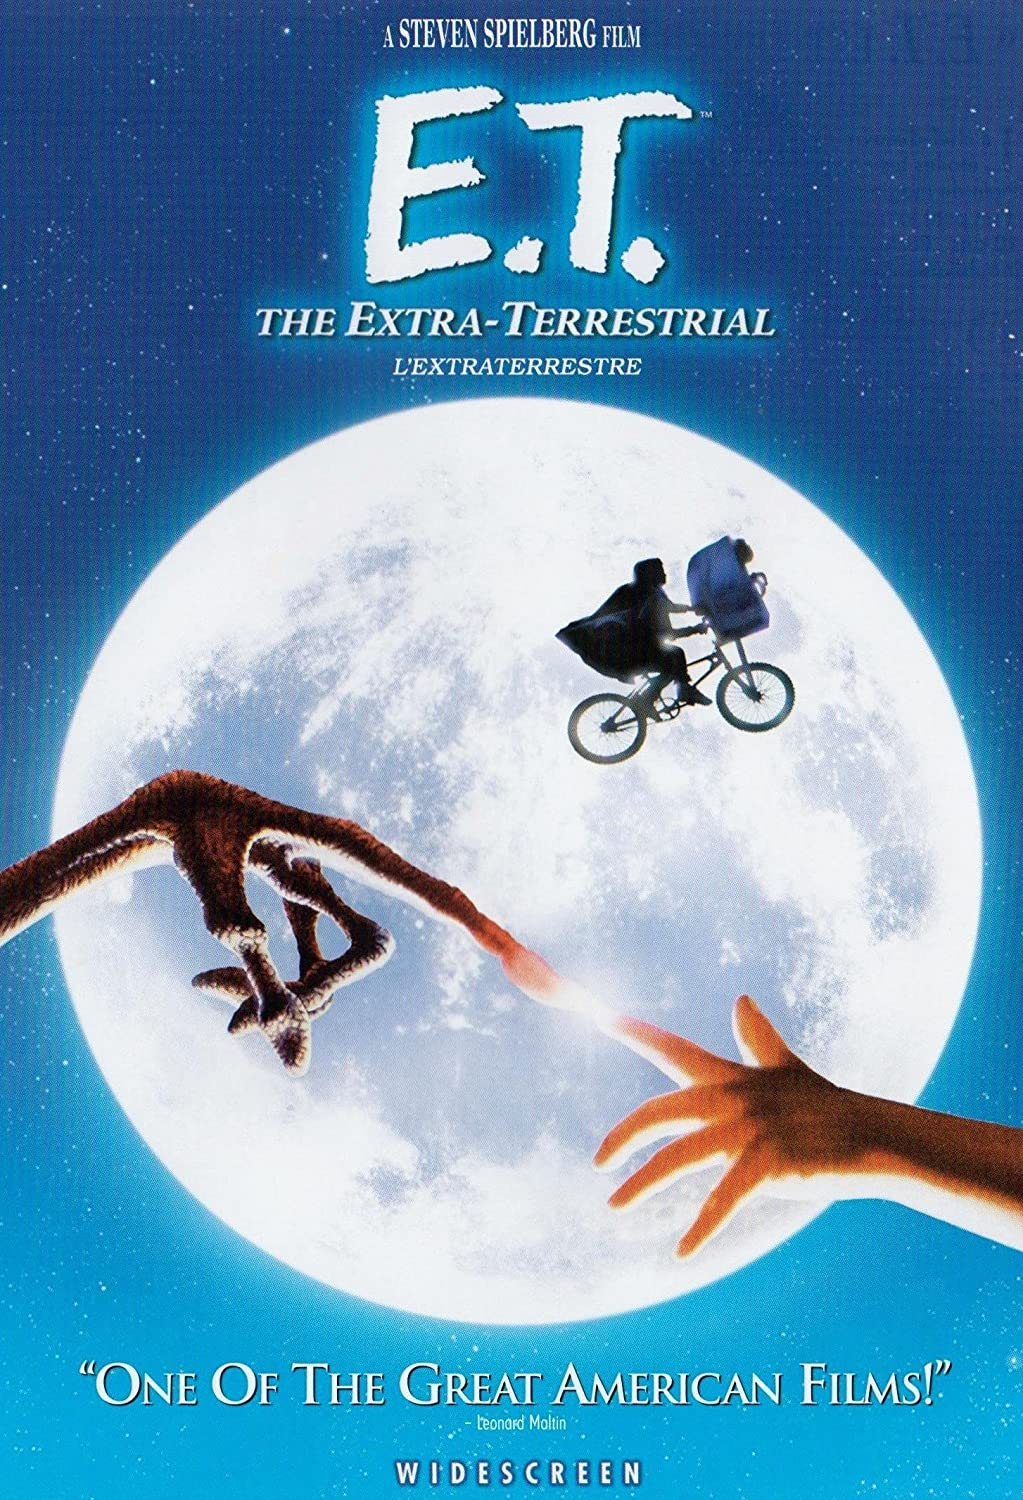
\includegraphics[height=1.25in,  width=1.0in]{images/ET-FU.jpg}}
\end{picture}
\end{frame}

%%%%%%%%%%%%%%%%%%%%%%%%%%%%%%%%%%%%%%%%%%%%%%%%%%%
%%%%%%%%%%%%%%%%%%%% Methods  %%%%%%%%%%%%%%%%%%%%%
%%%%%%%%%%%%%%%%%%%%%%%%%%%%%%%%%%%%%%%%%%%%%%%%%%%
\section{Methods}


\begin{frame}
\frametitle{Background}
\begin{itemize}
    \item Astronomers focus on finding chemical signs of life, not extraterrestrial intelligence
    \pause
    \begin{enumerate}
        \item Reasonable assumption. Intelligent life on Earth detectable only for
              100 years out of 4.5 billion years
        \pause
    \end{enumerate}
    \item Before we find life, we need to identify exoplanets candidates for life
    \pause
    \begin{enumerate}
        \item Want statistics on types of planets and understand how they form
        \pause
        \item Follow up good candidates with spectroscopy 
        \pause
        \item Use chemical and physical modelling to understand the possible signatures
        \pause
        \item Biased towards Earth-like life, since that is all we know.
    \end{enumerate}
\end{itemize}
\end{frame}


\begin{frame}
\frametitle{Jargon}
\begin{itemize}
    \item Light Year (ly) = $9.461\times 10^{12}$km
    \pause
    \item Exoplanet
    \pause
    \begin{enumerate}
        \item Planets NOT in our solar system
        \pause 
        \item Generally orbitting stars outside of our solar system.
        \pause
        \item 4 Types
        \pause
        \begin{itemize}
            \item[--] Gas Giant (100's $M_{E}$)
            \pause
            \item[--] Neptunian (10's $M_{E}$)
            \pause
            \item[--] Super-Earth (few $M_{E}$)
            \pause
            \item[--] Terrestrial ($\leq M_{E}$)
        \end{itemize}
        \pause
        \item Closest - Proxima Centari b - 4.25ly
        \pause
        \item Farthest - SWEEPS-11 in Sagittarius - 27700ly
    \end{enumerate}
\end{itemize}
\end{frame}


\begin{frame}
\frametitle{Jargon}
\begin{picture}(320,250) 
\visible<2->{\put(10, 60){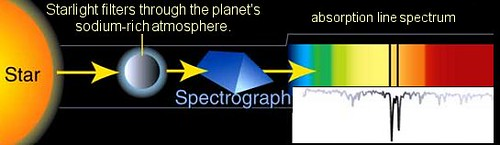
\includegraphics[height=1.2in]{images/spectra-PD.jpg}}}
\put(-20, 240){\begin{minipage}[t]{0.8 \linewidth}
{
\begin{itemize}
    \item Spectroscopy -
    \pause
    \begin{enumerate}
        \item Using light emmitted (or absorbed) by objects to determine their composition
        \pause
        \item E.g.
        \begin{itemize}
            \item[--] Using a prism to split white light into the colors of the rainbow.
            \pause
            \item[--] Rainbows
        \end{itemize}
    \end{enumerate}
\end{itemize}
}
\end{minipage}}
\end{picture}
\end{frame}


\begin{frame}
\frametitle{Jargon}
Angular Size
\pause
\begin{itemize}
    \item degree : 360 degrees in a circle
    \pause
    \item arcminute : 60 arcminutes in a degree
    \pause
    \item arcsecond : 60 arcsecond in a arcminute % 3600 arcseconds in a degree
\end{itemize}
\end{frame}



\begin{frame}
\frametitle{4 Common Ways to Find a Planet}
\begin{enumerate}
    \item Radial Velocity Method
        \pause
        \begin{itemize}
            \item Watching for stars `wobbling' spectroscopically
            \pause
            \item 915 planets
            \pause
            \item Advantage : Planets don't have to be in line with our line-of-sight
            \pause
            \item Show video
        \end{itemize}
    \pause
    \item Transit Method
        \pause
        \begin{itemize}
            \item Watching for occluding 
            \pause
            \item 3759 planets
            \pause
            \item Advantage : Really `easy' to do with surveys (e.g. Kepler)
            \pause
            \item Disadvantage : Planets must be along the line-of-sight
            \pause
            \item Show video
        \end{itemize}
\end{enumerate}
\end{frame}


\begin{frame}
\frametitle{4 Common Ways to Find a Planet}
\begin{picture}(320,250) 
\visible<2->{\put(190, 70){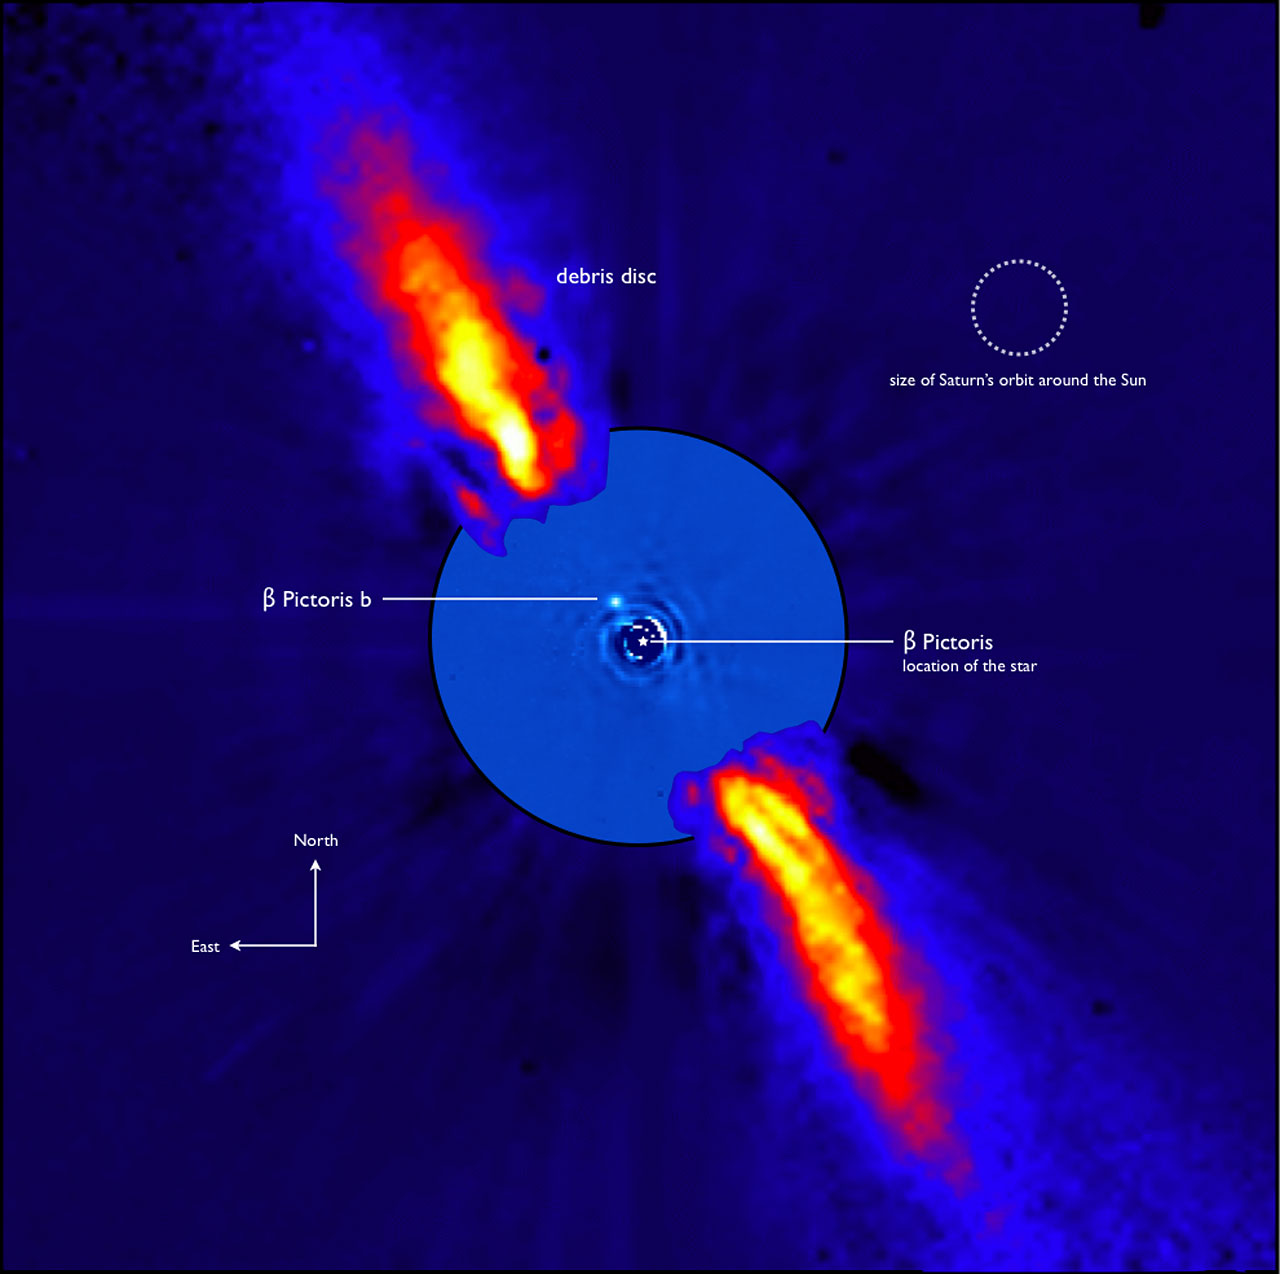
\includegraphics[height=2.25in]{images/beta-pictoris-b-FU.jpg}}}
\put(-20, 240){\begin{minipage}[t]{0.7 \linewidth}
{
\begin{enumerate}
    \setcounter{enumi}{2}
    \item Direct Imaging Method (amazing)
        \pause
        \begin{itemize}
            \item Mildly Miraculous 
                \pause
                \begin{itemize}
                    \item[--] Seems to defy the optical resolution equation $\theta = 1.22 \frac{\lambda}{D}$
                    % Beta Pictoris b
                    % https://www.eso.org/public/archives/releases/sciencepapers/eso0842/eso0842.pdf
                    % \lambda = 3600e-6 , D=8, \theta = 1.22 * 3600e-6/8 = 0.00055rads
                    % sin(\theta) = o/h = 8AU / 63ly = 1.12e12 / 5.96e17 = 1.88e-6, small angle \theta = 1.88e-6rads
                    % Analogy : CBUS -> CHICAGO = 275miles = 442570m, like resolving 
                    %           o = h sin(\theta) = 442570 * sin(1.88e-6) = 0.8m
                    % Like resolving a car tire in chicago
                \end{itemize}
            \pause
            \item Advantage : Planets don't have to be in line with our line-of-sight
            \pause
            \item Disadvantage / Advantage : Primarily young gas giants (few million years old)
            \pause
            \item Disadvantage : Really hard to do
            \pause
            \item 58 planets
            \pause
            \item Show HR\_8799\_Orbiting\_Exoplanets.gif
        \end{itemize}
\end{enumerate}
}
\end{minipage}}
\end{picture}
\end{frame}


\begin{frame}
\frametitle{4 Common Ways to Find a Planet}
\begin{enumerate}
    \setcounter{enumi}{3}
    \item Gravitational Microlensing Method
        \pause
        \begin{itemize}
            \item Advantage : Can spot planets NOT bound to a star (i.e. free-floating)
            \pause
            \item Disadvantage : Follow up observations are hard
            \pause
            \item 124 planets
            \pause
            \item Show video
        \end{itemize}
\end{enumerate}
\end{frame}


%%%%%%%%%%%%%%%%%%%%%%%%%%%%%%%%%%%%%%%%%%%%%%%%%%%
%%%%%%%%%%%%%%%%%% Experiments %%%%%%%%%%%%%%%%%%%%
%%%%%%%%%%%%%%%%%%%%%%%%%%%%%%%%%%%%%%%%%%%%%%%%%%%
%\section{Experiments}
\begin{frame}
\frametitle{Experiments - Kepler}
\begin{picture}(320,250) 
\visible<1->{\put(200, 100){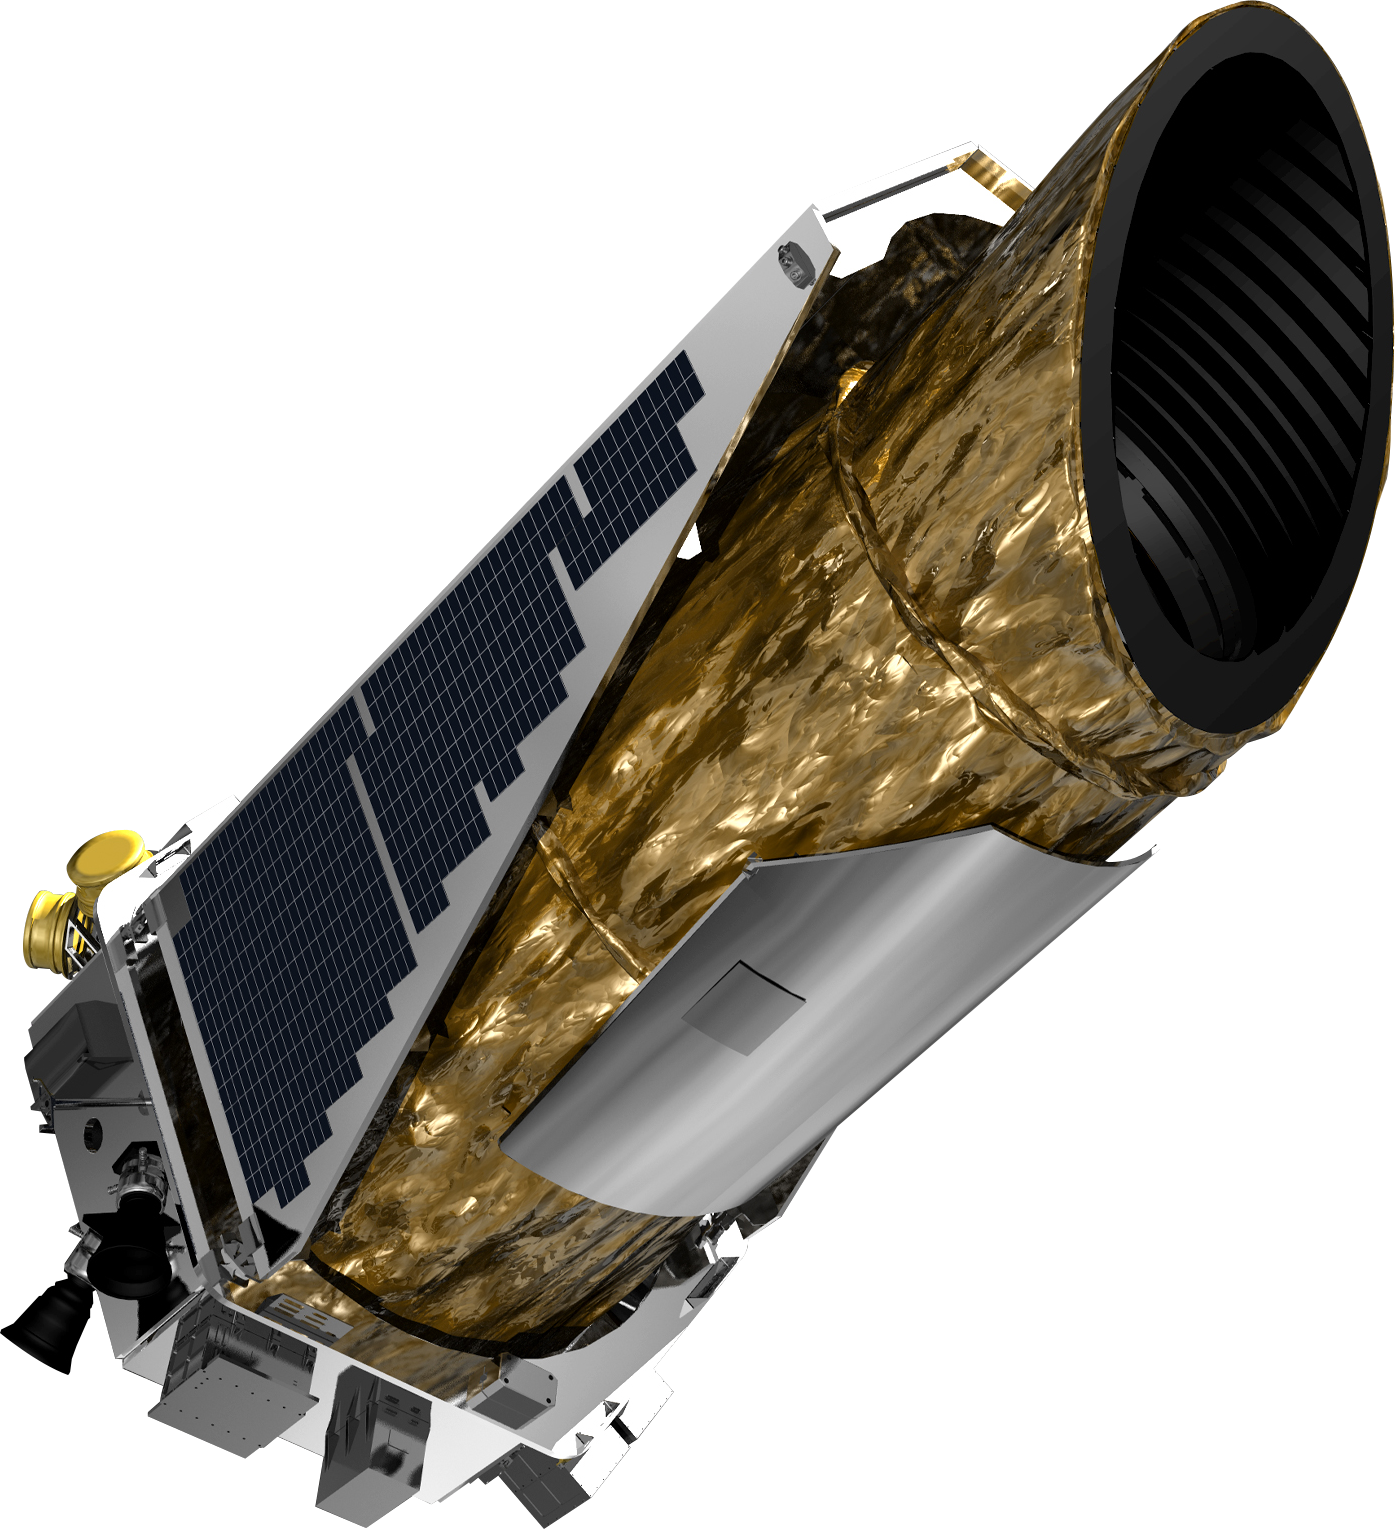
\includegraphics[height=1.5in]{images/kst-PD.png}}}
\put(-20, 230){\begin{minipage}[t]{0.7 \linewidth}
{Kepler Space Telescope (2009-2018)
% Mention irony
\begin{itemize}
    \item Telescope mirror = 0.95m, Field of view = 115 $\text{deg}^{2}$
    \pause 
    \item Orbits Sun, NOT earth
    \pause 
    \item Continually monitored 530,000 stars in Cygnus, Lyra and Draco
    \pause 
    \item Used Transit method
    \pause 
    \item Detected 2662 planets
    \pause 
    \item Biased towards large planets with short periods.
    \pause 
    \item Most planets too far to chemically characterize
\end{itemize}}
\end{minipage}}
\end{picture}
\end{frame}


\begin{frame}
\frametitle{Experiments - TESS}
\begin{picture}(320,250) 
\visible<1->{\put(200, 100){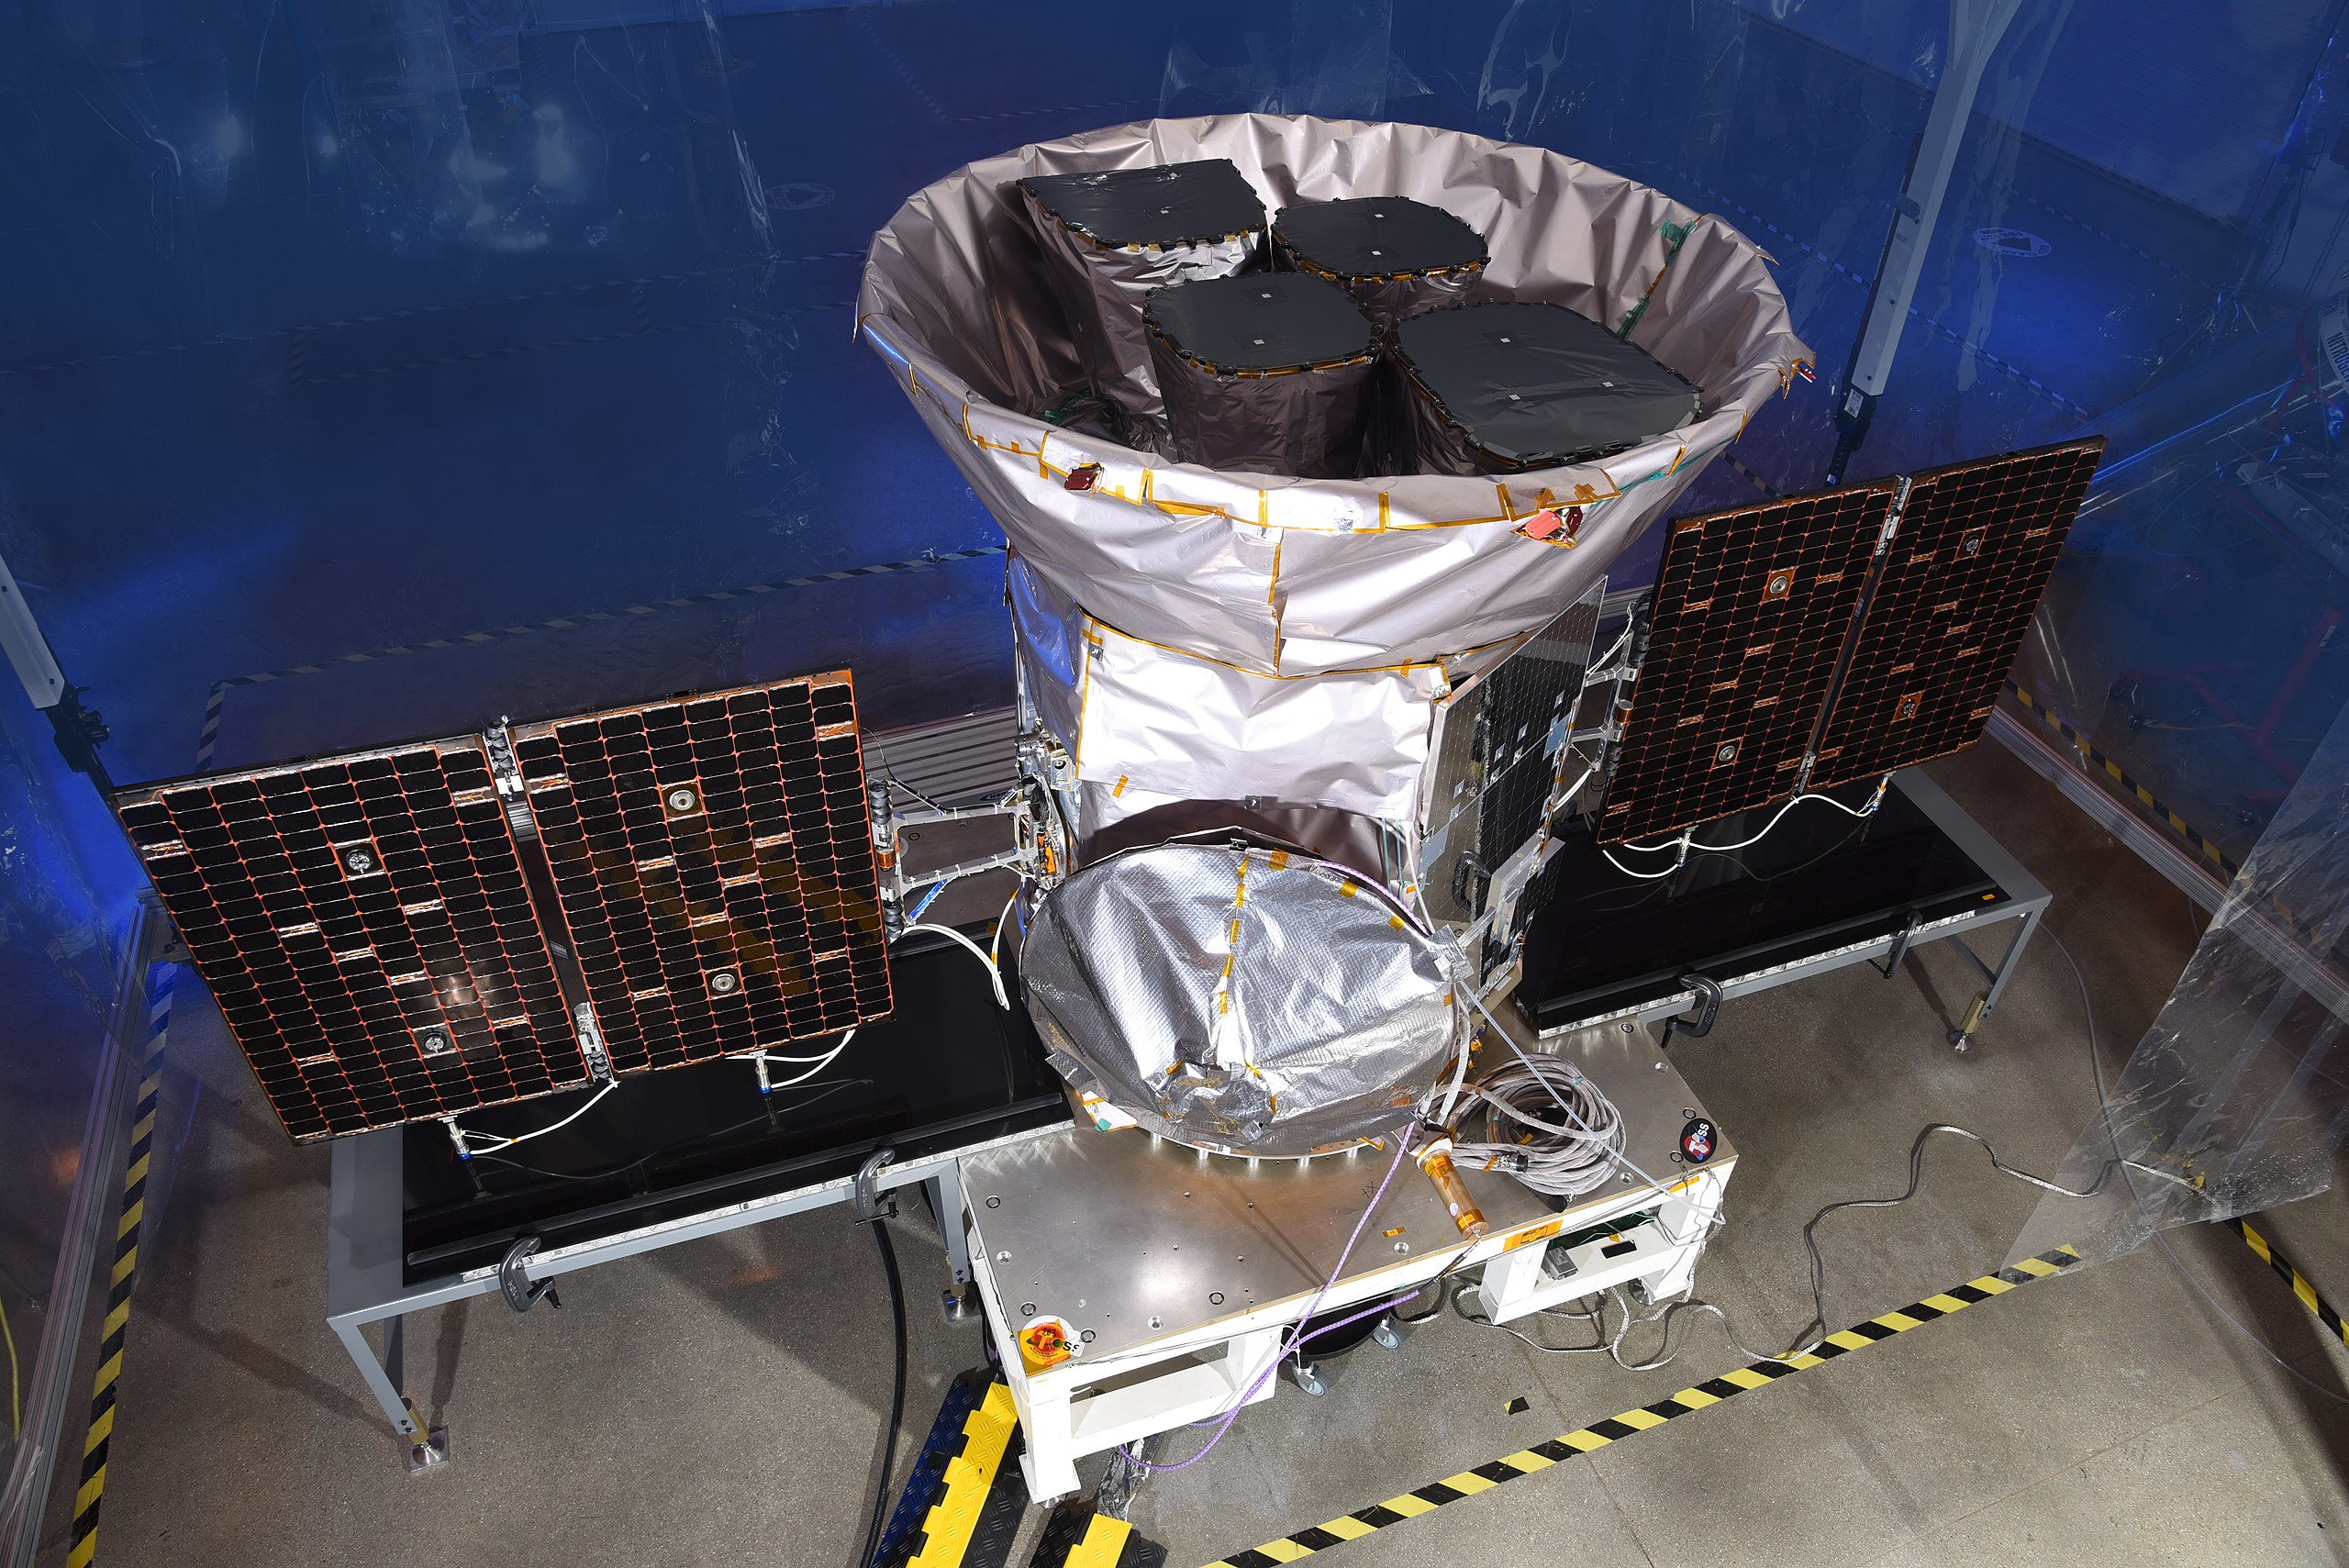
\includegraphics[height=1.2in]{images/TESS-PD.jpg}}}
\put(-20, 240){\begin{minipage}[t]{0.7 \linewidth}
{Transiting Exoplanet Survey Satellite (2018-current)
\begin{itemize}
    \item 4 camera's with 4" diameter lense, Field of view = 2300 $\text{deg}^{2}$
    \pause 
    \item Observes 85\% of the sky. Survey 200,000 brightest stars
    \pause 
    \item Provides targets for detailed spectroscopy for James Webb Space Telescope
    \pause 
    \item Primary mission is to survey brightest stars near Earth
    \pause 
    \item Used Transit method
    \pause 
    \item Detected 2600 exoplanet candidates, 122 confirmed
\end{itemize}}
\end{minipage}}
\end{picture}
\end{frame}


\begin{frame}
\frametitle{Experiments - JWST}
\begin{picture}(320,250) 
\visible<1->{\put(200, 100){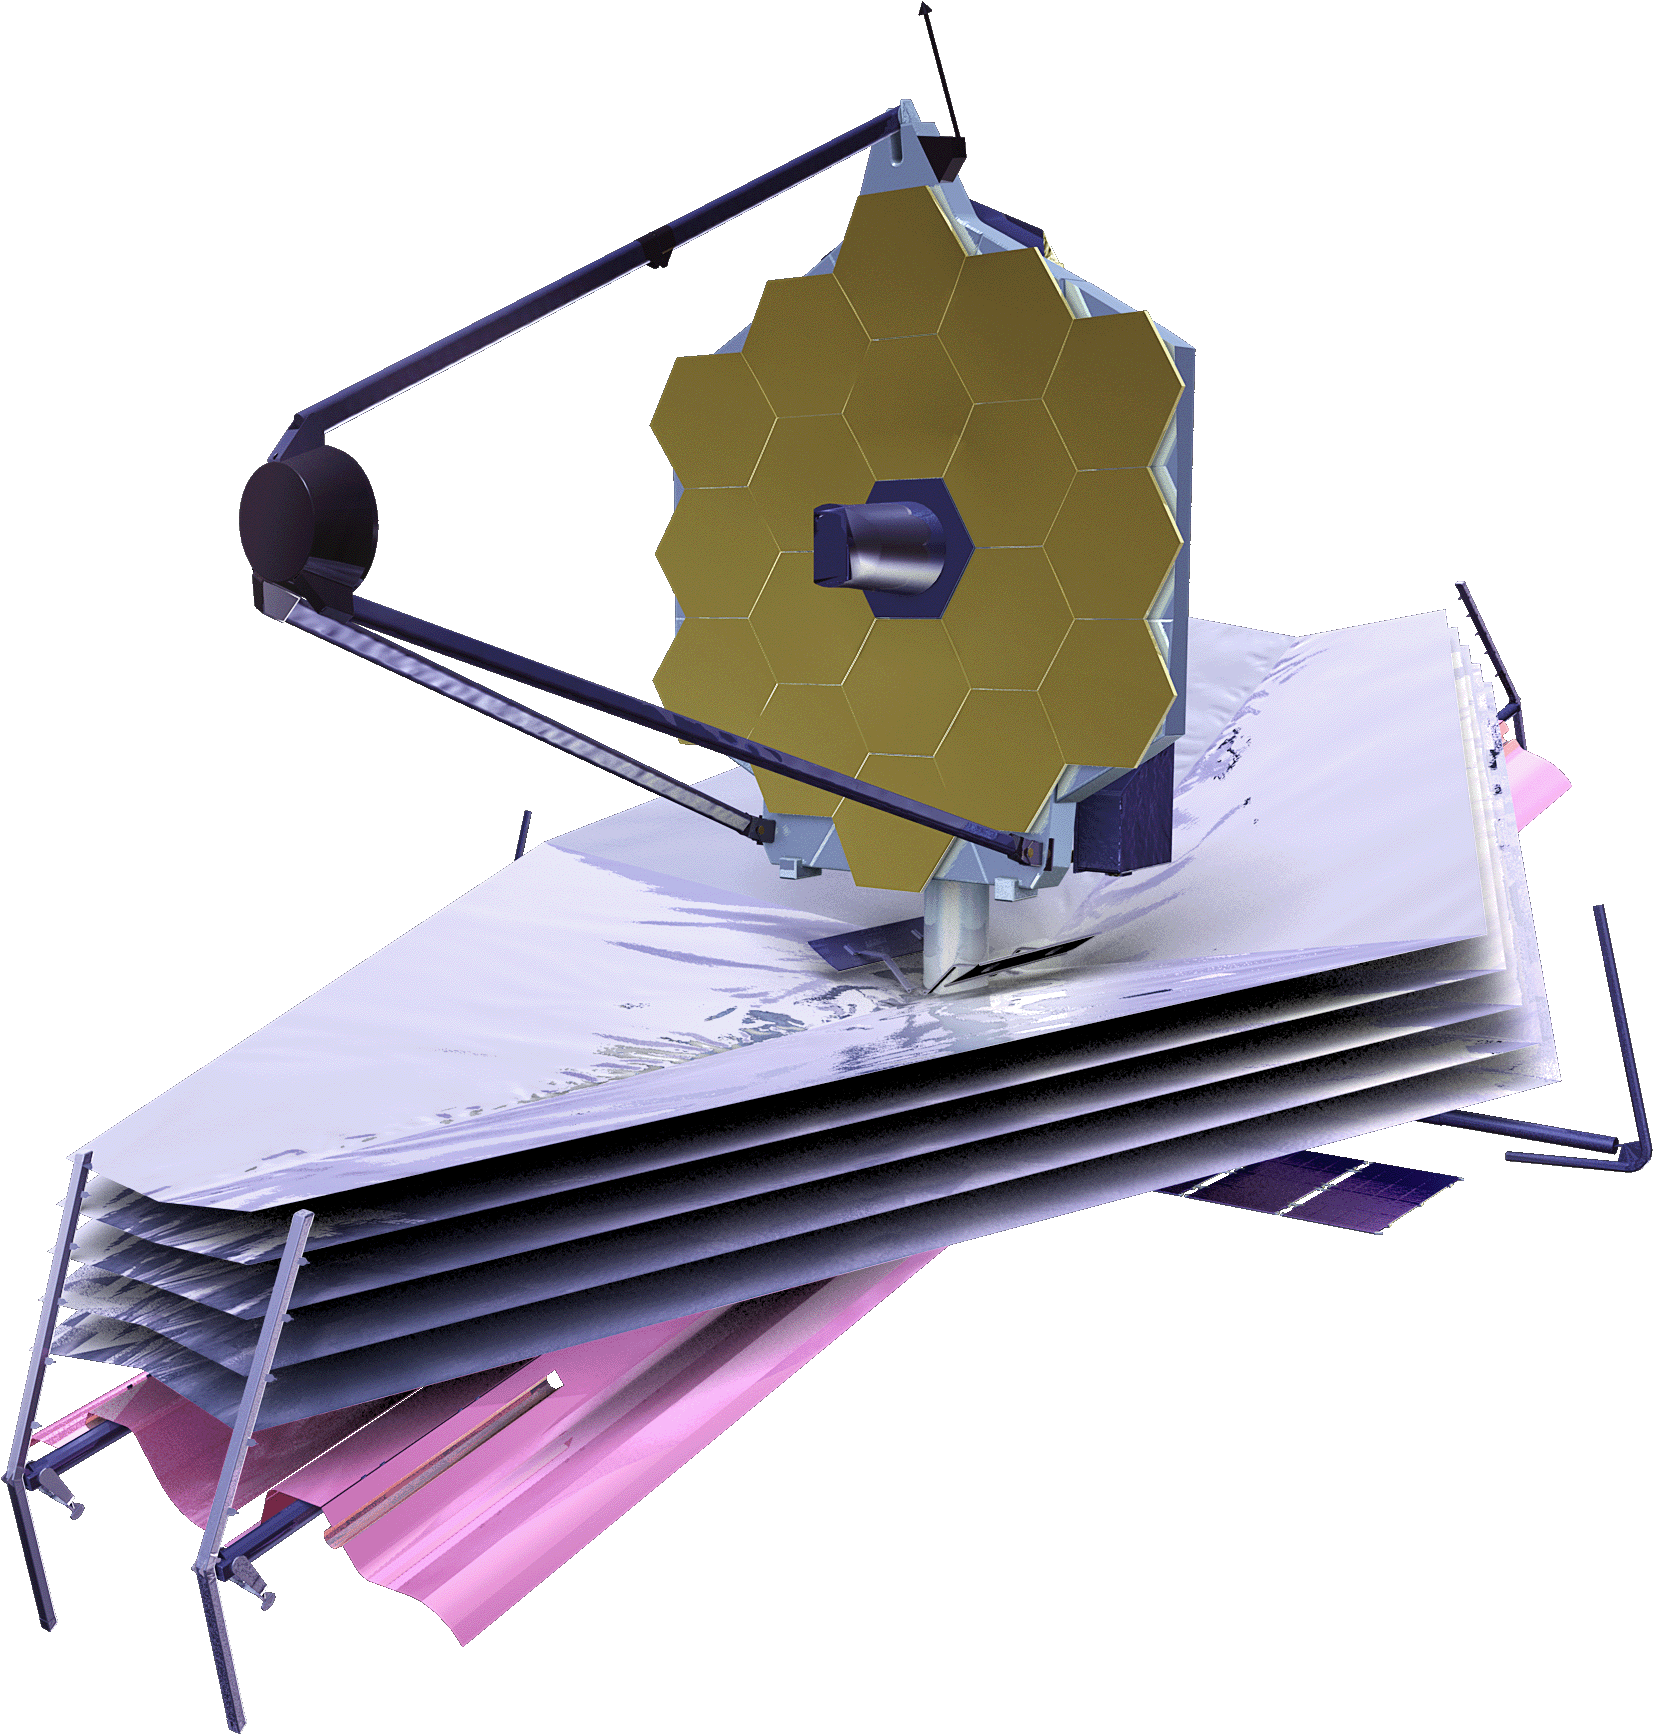
\includegraphics[height=1.5in]{images/JWST-PD.png}}}
\put(-20, 230){\begin{minipage}[t]{0.6 \linewidth}
{James Web Space Telescope (2022-current)
\begin{itemize}
    \item Infrared telescope with 6.5m mirror, Field of view = 0.0025 $\text{deg}^{2}$
    \pause 
    \item Small field of view
    \pause 
    \item Large collection of ligth
    \pause 
    \item Not a dedicated mission
    \pause 
    \item Used Transit method
    \pause 
    \item Should be able to characterize atmospheres around rocky, Earth-like planets
\end{itemize}}
\end{minipage}}
\end{picture}
\end{frame}


\begin{frame}
\frametitle{Experiments - Square Kilometer Array}
\begin{picture}(320,250) 
\visible<1->{\put(200, 100){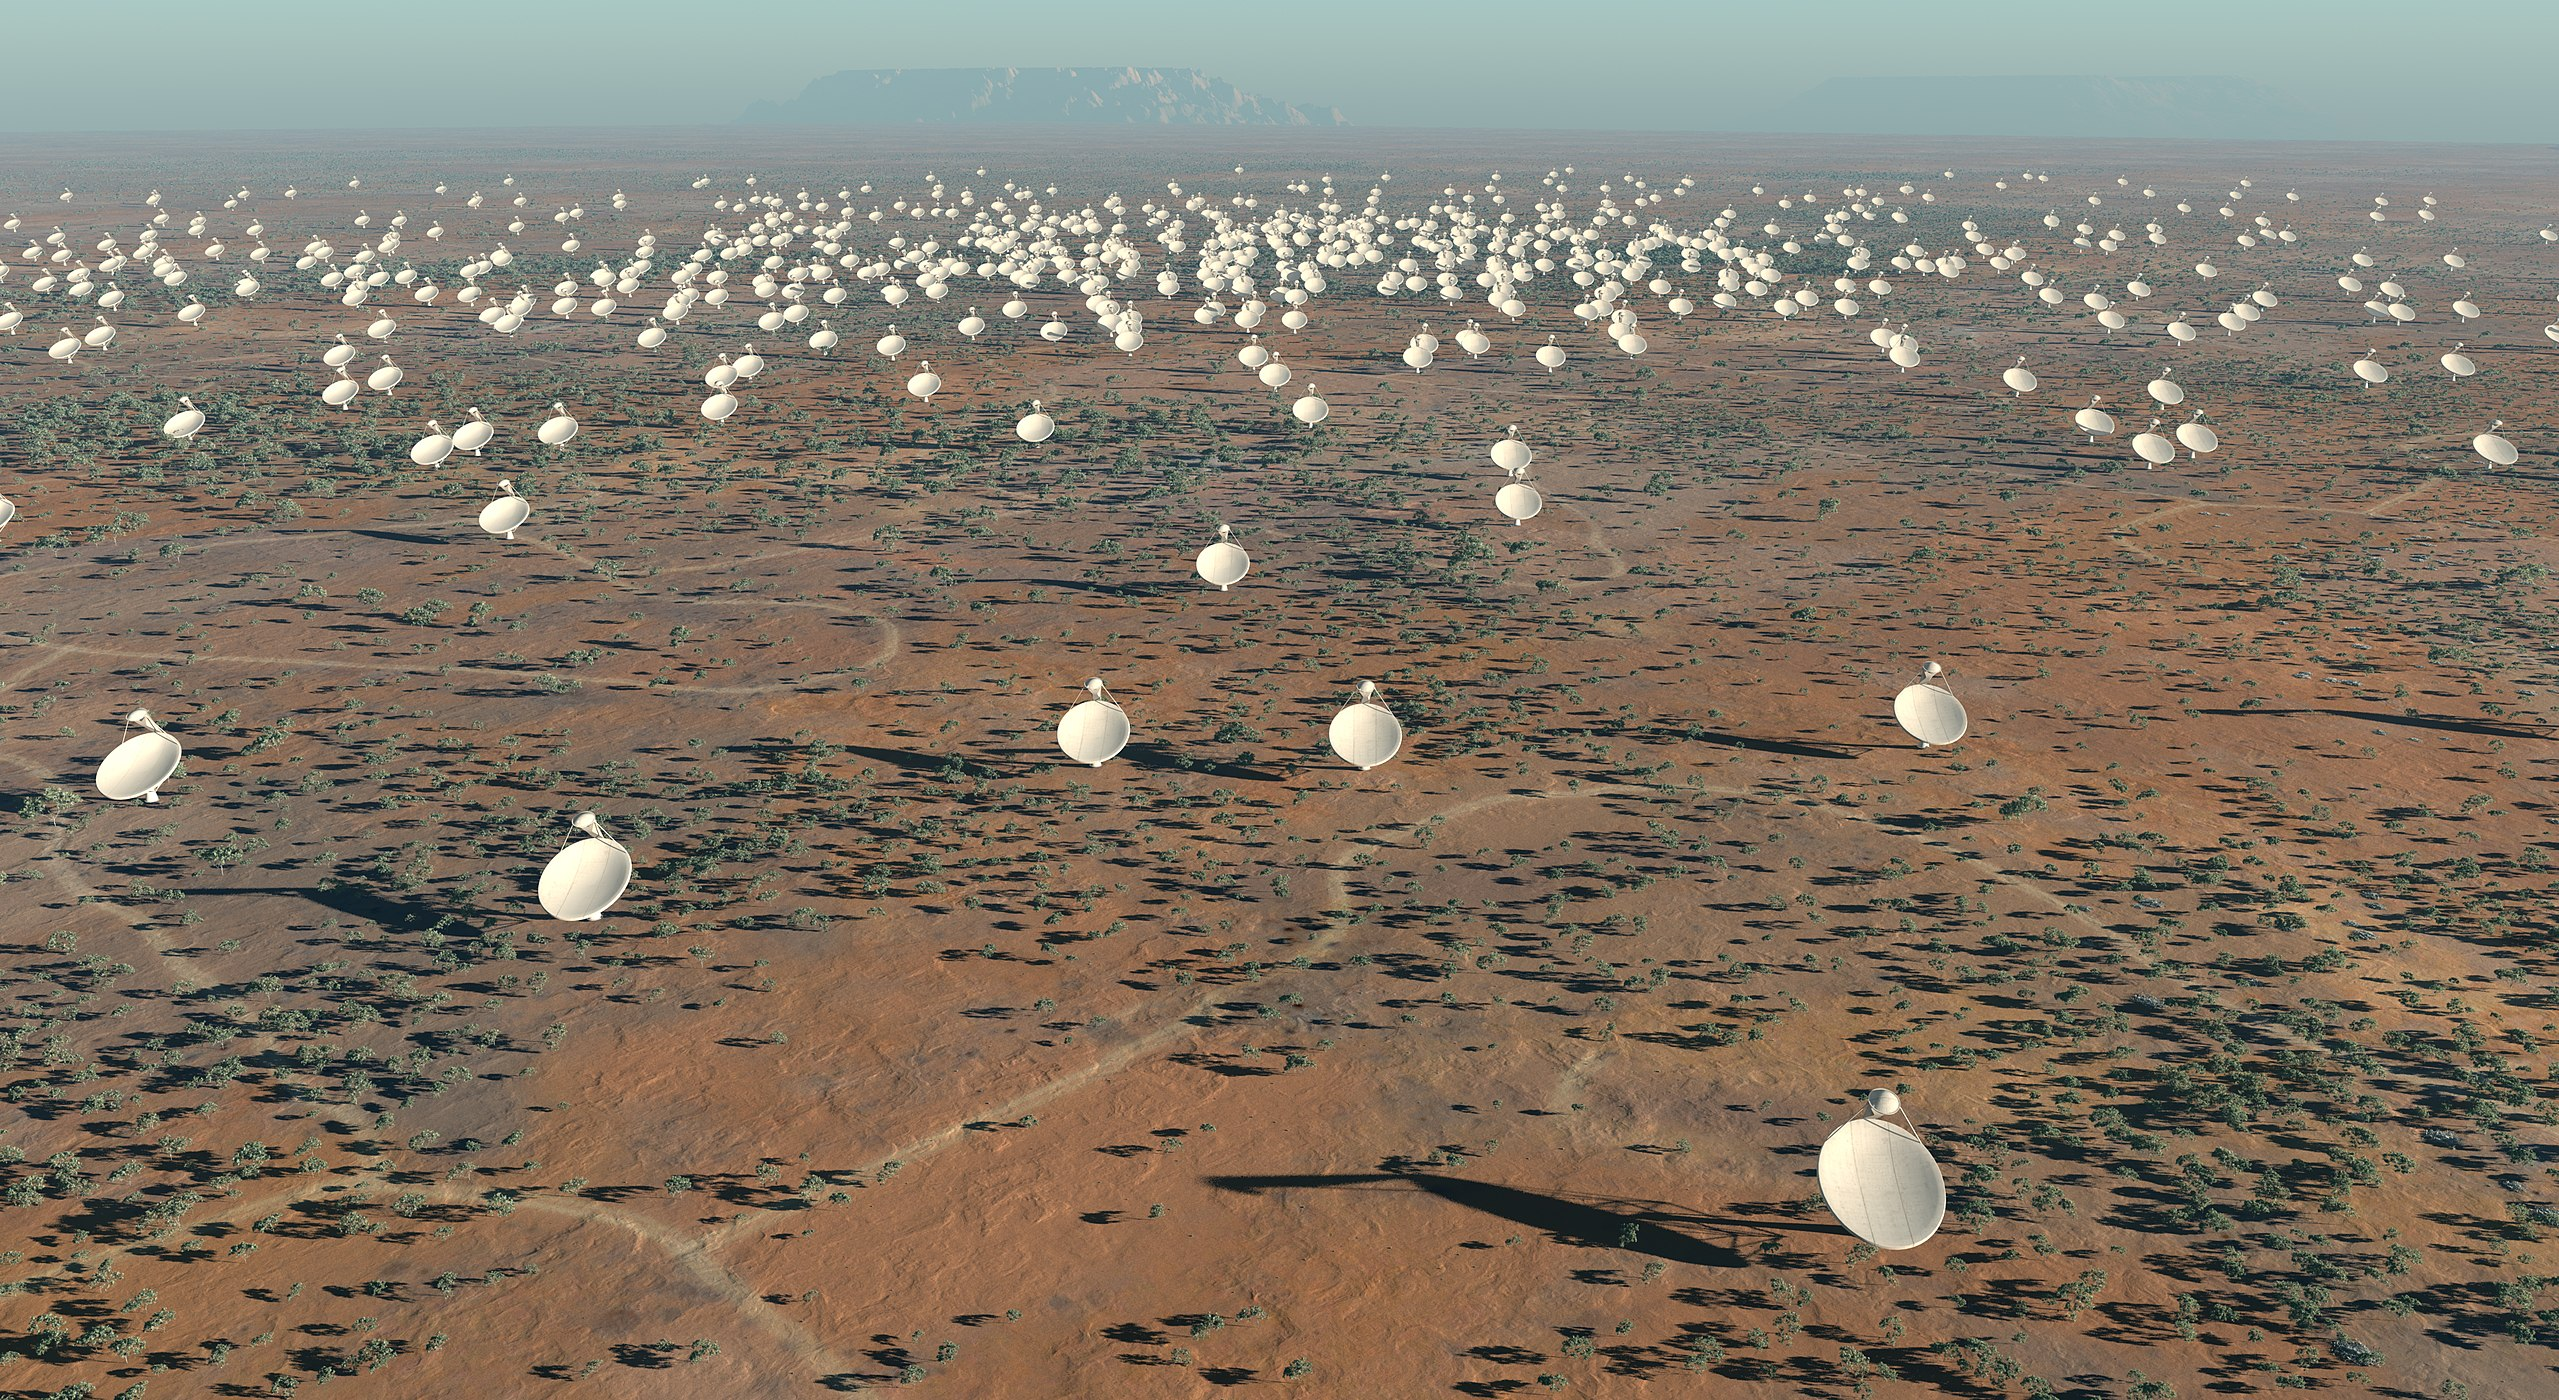
\includegraphics[height=1.25in]{images/ska-cc-by-3.jpg}}}
\put(-20, 240){\begin{minipage}[t]{0.7 \linewidth}
{Square Kilometer Array (Future)
\begin{itemize}
    \item Radio telescope with 1$\text{km}^{2}$ effective collecting area
    \pause 
    \item Made of thousands 12m radio dishes
    \pause
    \item Located in South Africa
    \pause 
    \item First telescope to be explicitly designed with SETI in mind
    \pause 
    \item Could detect extraterrestrial long range aircraft radar out to 200ly
    \begin{enumerate}
        \item Includes 10,000 stars
    \end{enumerate}
    \pause 
    \item Detect extraterrestrial planetary radar from thousands of light years away
    \begin{enumerate}
        \item Includes millions of stars
    \end{enumerate}
\end{itemize}}
\end{minipage}}
\end{picture}
\end{frame}

%%%%%%%%%%%%%%%%%%%%%%%%%%%%%%%%%%%%%%%%%%%%%%%%%%%
%%%%%%%%%%%%%%%%%% Signs of Life %%%%%%%%%%%%%%%%%%%%
%%%%%%%%%%%%%%%%%%%%%%%%%%%%%%%%%%%%%%%%%%%%%%%%%%%
\section{Life}

\begin{frame}
\frametitle{Signs of Life - Where to Look}
\begin{picture}(320,250) 
\visible<1->{\put(160, 65){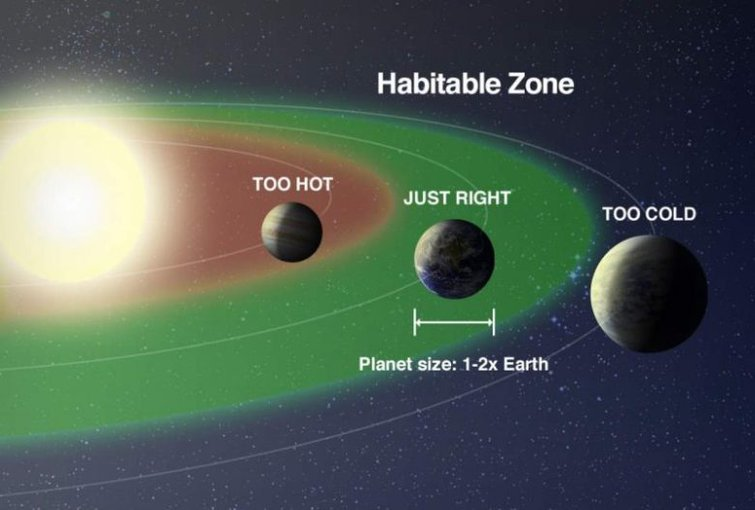
\includegraphics[height=1.5in]{images/habitable-zone-FU.jpg}}}
\put(-20, 240){\begin{minipage}[t]{0.7 \linewidth}
{
Habitable Zone : 
\begin{itemize}
    \item Liquid water can exist in this regime
    \pause
    \item In our solar system this is from Venus to Mars
    \pause
    \item Depends on star and planetary composition
\end{itemize}
}
\end{minipage}}
\end{picture}
\end{frame}

\begin{frame}
\frametitle{Signs of Life - What to Look for}
Plant life (photosynthesis)
\begin{itemize}
    \item $\text{O}_{2}$
    \pause
    \item $\text{CO}_{2}$
    \pause
    \item $\text{CH}_{4}$
    \pause
\end{itemize}

Animal life (intelligent life) : 
\begin{itemize}
    \item $\text{NO}_{X}$
    \pause
    \item Air pollution / smog
    \pause
    \item Radio emission
    % Mention SKA
\end{itemize}
\end{frame}

%%% Experiments in a jar
% SWEEPS https://en.wikipedia.org/wiki/Sagittarius_Window_Eclipsing_Extrasolar_Planet_Search
%\section{Signatures of Life} %

%%%%%%%%%%%%%%%%%%%%%%%%%%%%%%%%%%%%%%%%%%%%%%%%%%%
%%%%%%%%%%%%%%% Intelligent Life %%%%%%%%%%%%%%%%%%
%%%%%%%%%%%%%%%%%%%%%%%%%%%%%%%%%%%%%%%%%%%%%%%%%%%
%\section{Intelligent Life}
\begin{frame}
\frametitle{Drake Equation}
% https://www.seti.org/drake-equation-index
$$ N = R_{*} \cdot f_{p} \cdot n_{e} \cdot f_{L} \cdot f_{i} \cdot f_{c} \cdot L$$
\begin{itemize}
    \item $N$ : number of detectable civilizations 
    \item $R_{*}$ : Rate of formation of stars suitable for intelligent life
    \item $f_{p}$ : Fraction of stars with planetary systems
    \item $n_{e}$ : Number of planets per solar system with an environment suitable for life
    \item $f_{L}$ : Fraction of suitable planets where life occurs
    \item $f_{i}$ : Fraction of planets where intelligent life emerges
    \item $f_{c}$ : Fraction of civilizations that develop technology that produces signal
    \item $L$     : Life span of technologically advanced civilizations
\end{itemize}
\end{frame}


\begin{frame}
\frametitle{Drake Equation}
% https://www.seti.org/drake-equation-index
$$ N = R_{*} \cdot f_{p} \cdot n_{e} \cdot f_{L} \cdot f_{i} \cdot f_{c} \cdot L$$
Selecting reasonable values (for Milky Way): 
\begin{itemize}
    \item $N$ : unknown
    \item $R_{*} \sim 2$
    \item $f_{p} = 1$
    \item $n_{e} = 0.5$ % per https://www.nasa.gov/feature/ames/kepler-occurrence-rate
    \item $f_{L} = \text{unknown} \leftarrow $ Active research
    \item $f_{i} = \text{unknown}$
    \item $f_{c} = \text{unknown}$ 
    \item $L     = \text{unknown}$ 
\end{itemize}
\pause
$$ N = 1.0 \cdot f_{L} \cdot f_{i} \cdot f_{c} \cdot L$$
\end{frame}


%%%%%%%%%%%%%%%%%%%%%%%%%%%%%%%%%%%%%%%%%%%%%%%%%%%
%%%%%%%%%%%%%%% Ain't so special %%%%%%%%%%%%%%%%%%
%%%%%%%%%%%%%%%%%%%%%%%%%%%%%%%%%%%%%%%%%%%%%%%%%%%
\section{Earth isn't so special}
\begin{frame}
\frametitle{Our Solar System}
Our Solar System : 
\begin{itemize}
    \item Our star is a run-of-the mill Main Sequence star
    \pause
    \item Sun will last about 10 billion years
    \pause
    \item Chemical composition is similar to many stars 
    \pause
    \begin{enumerate}
        \item Planets form from same dust / molecular cloud as star
        \pause
    \end{enumerate}
    \item ``Copernican Principle"
    \pause
    \begin{enumerate}
        %\item ``At large enough scale, the univeres appears homogeneous in all directions"
        %\pause 
        \item Interpret as : ``We don't live is a special place (e.g. star, planet, location)" 
        \pause
        %\item Doesn't quite apply here, but the style of thinking does
        %\pause
        \item Extrapolated : ``There is nothing special about where we are. If life occurs somewhere, it likely occurs everywhere"
        \pause
        \begin{itemize}
            \item[--] Throughout astronomy's history we've seen that if we think something can occur (e.g. black holes, white dwarfs, etc.), it frequently does.
        \end{itemize}
    \end{enumerate}
\end{itemize}
\end{frame}

%\begin{frame}
%\frametitle{Mass-Orbit Relation (2018)}
%\begin{picture}(320,250) 
%\put(10, 100){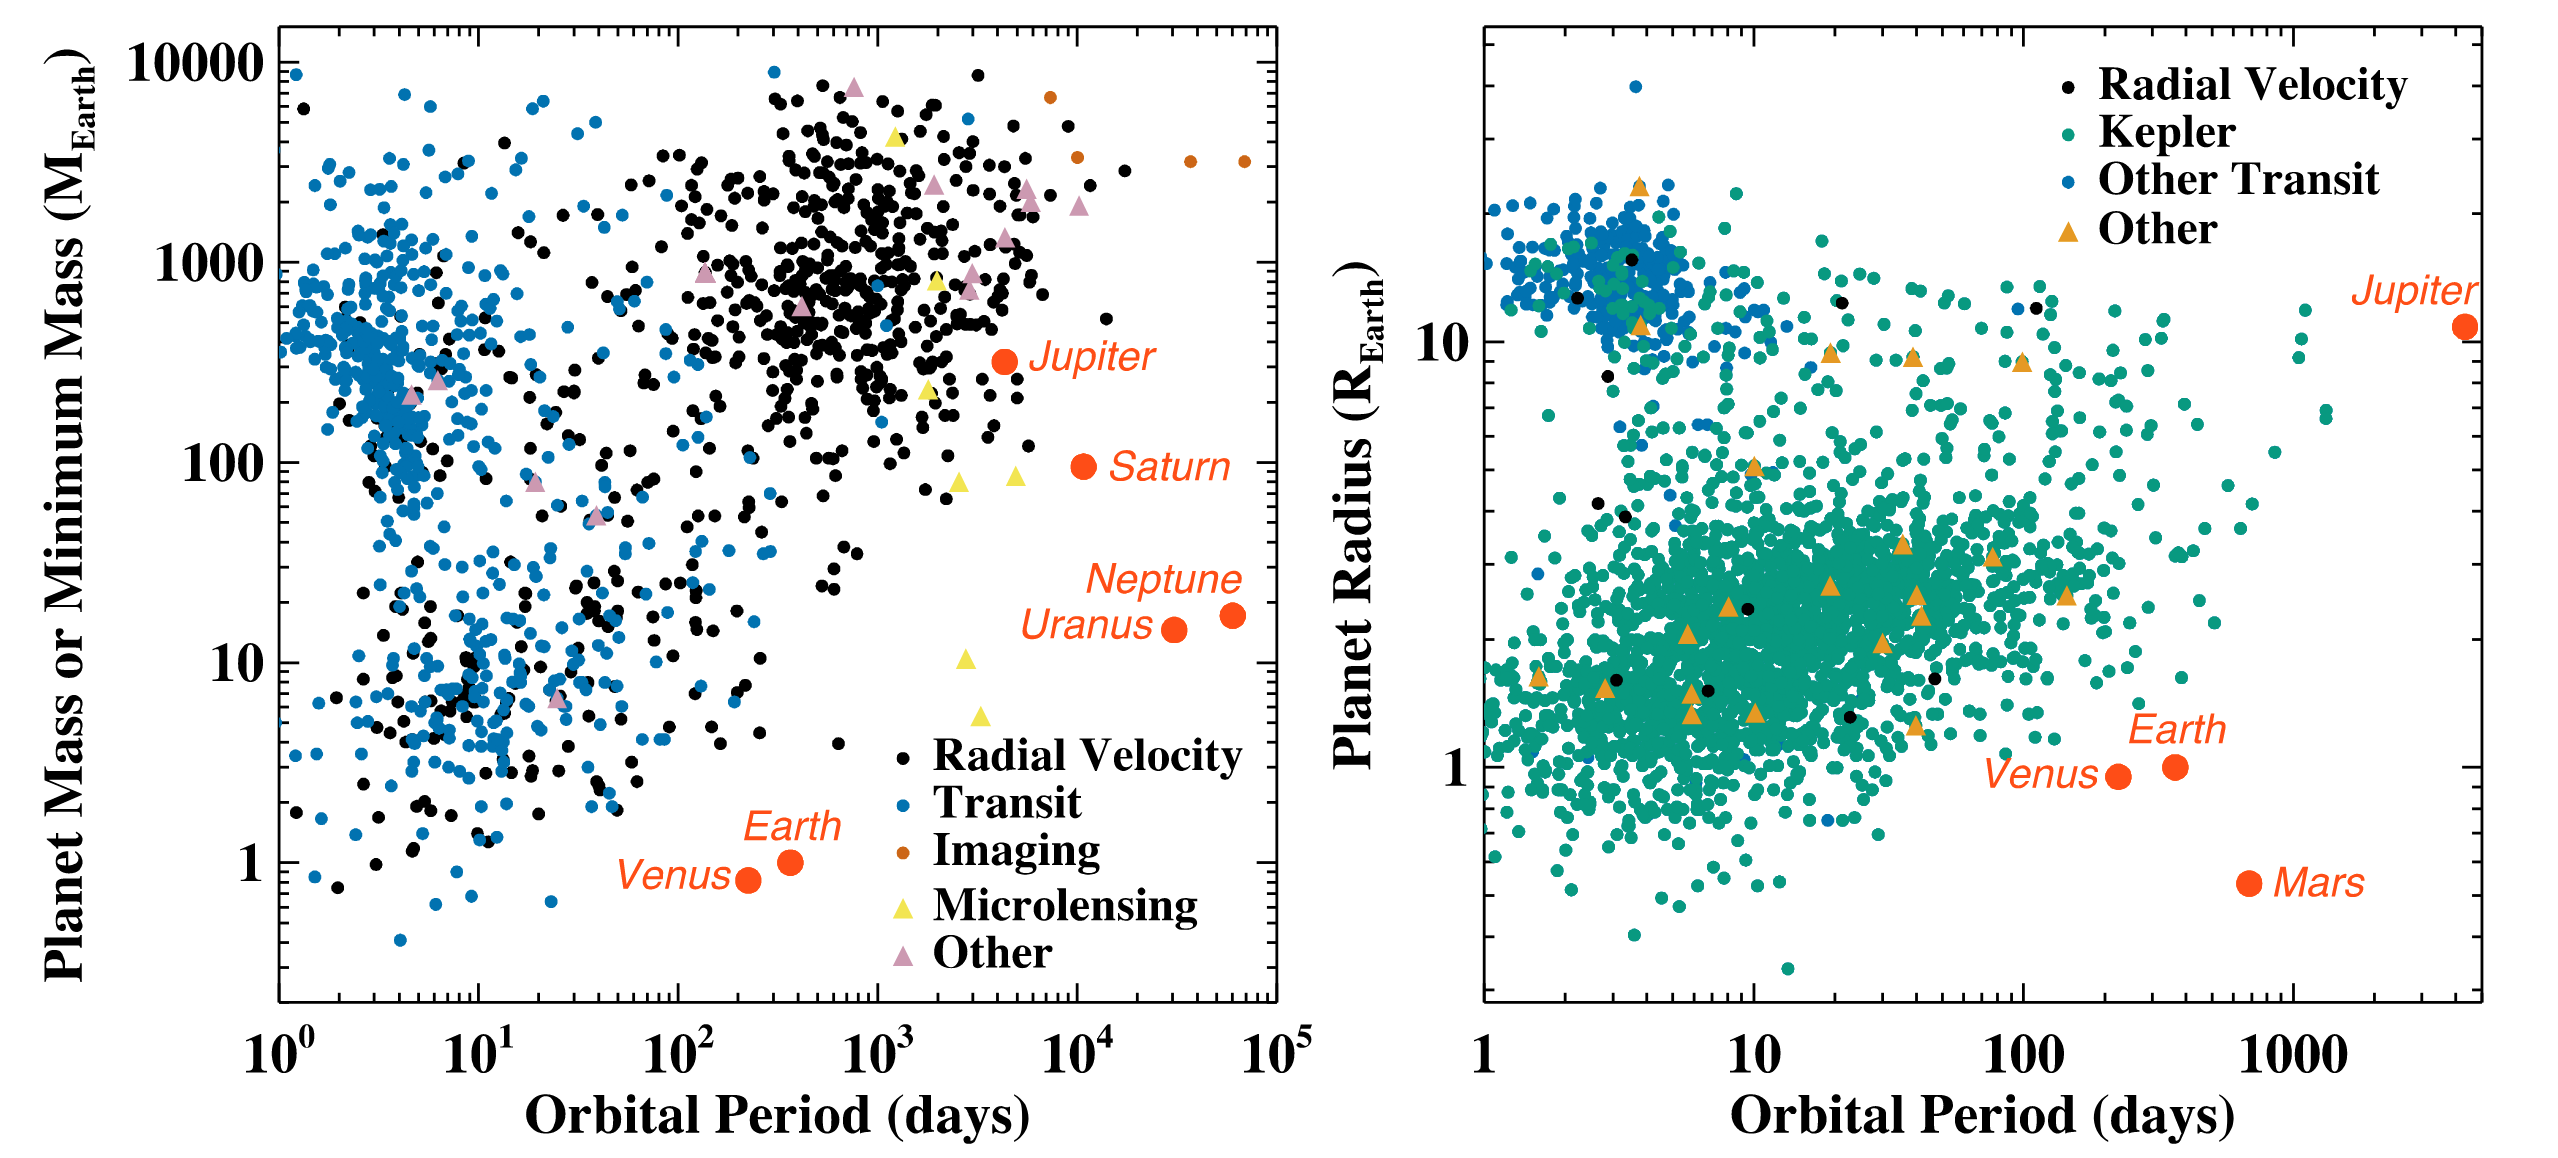
\includegraphics[width=3.75in]{images/mass-orbit-PD.png}}
%\end{picture}
%\end{frame}

\begin{frame}
\frametitle{Statistics}
\begin{picture}(320,250) 
\visible<1-4>{\put(75, 55){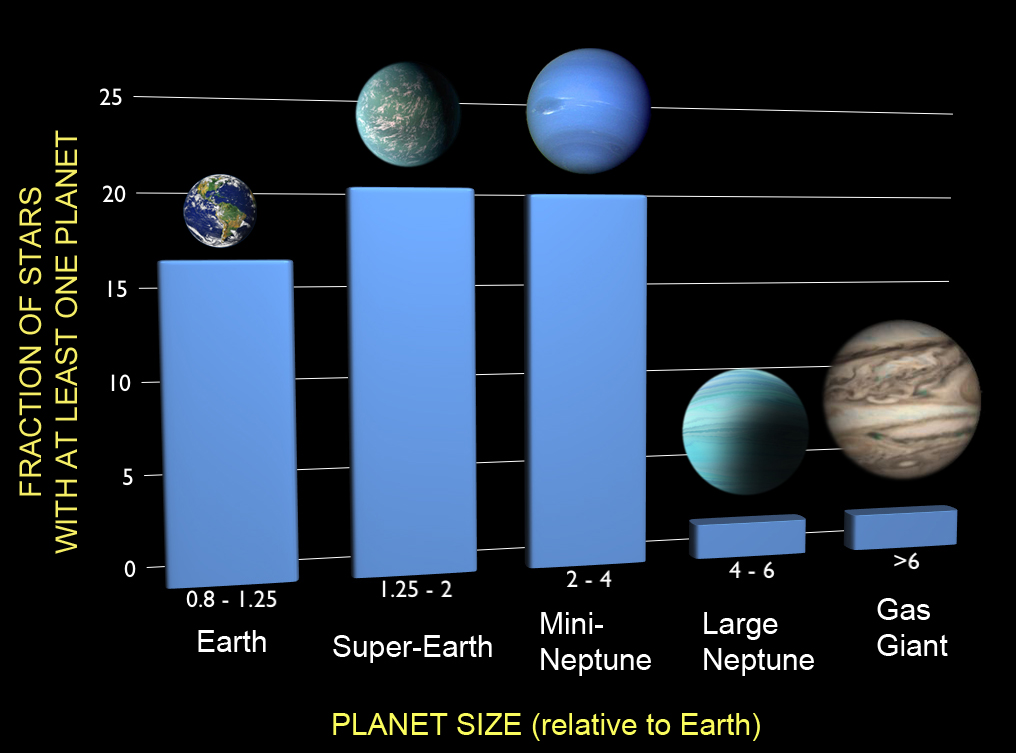
\includegraphics[height=1.7in]{images/exoplanet-size.jpg}}}
\visible<5>{\put(20, 55){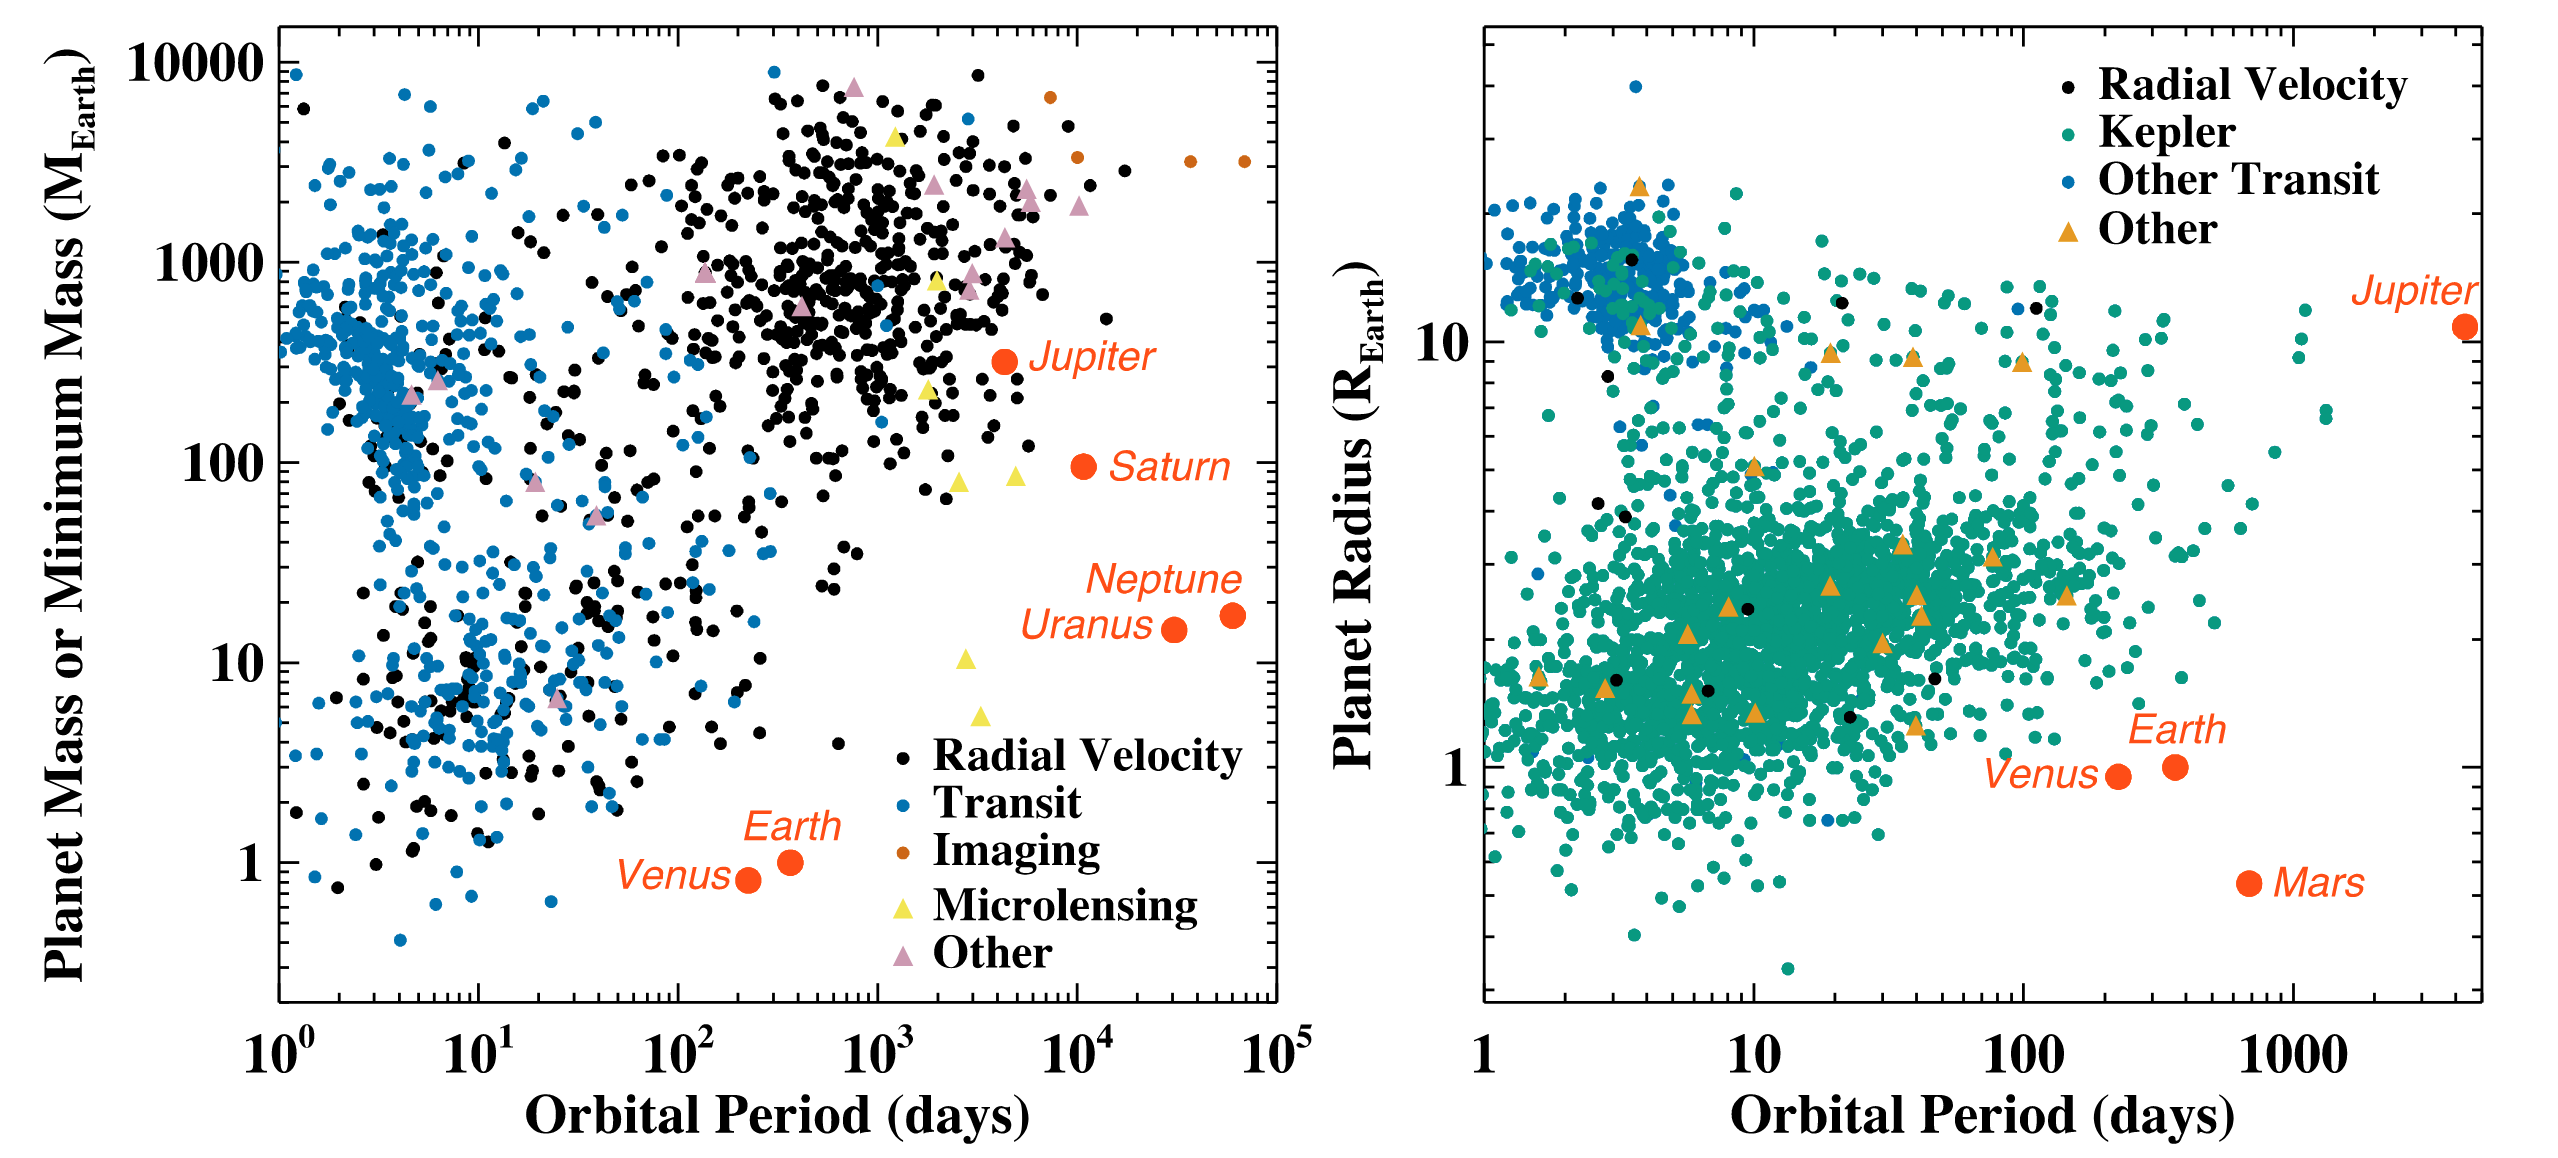
\includegraphics[width=3.75in]{images/mass-orbit-PD.png}}}
\put(-20, 240){\begin{minipage}[t]{0.8 \linewidth}
{Stars : 
\begin{itemize}
    \item 100's billions of stars, 90\% like our Sun
    %\pause
    %\item 90\%+ are like our sun    % Using Mo p 442 integrating Kroupa IMF from 1.2 - 0.5, eqn 9.42 and 9.33
    \pause
\end{itemize}
Planets : 
% https://www.nasa.gov/mission_pages/kepler/main/index.html
\begin{itemize}
    \pause
    \item Every star likely has more than one planet
    \pause
\end{itemize}}
\end{minipage}}
\end{picture}
\end{frame}


\begin{frame}
\frametitle{Fermi Paradox}
\begin{picture}(320,250) 
\put(-20, 55){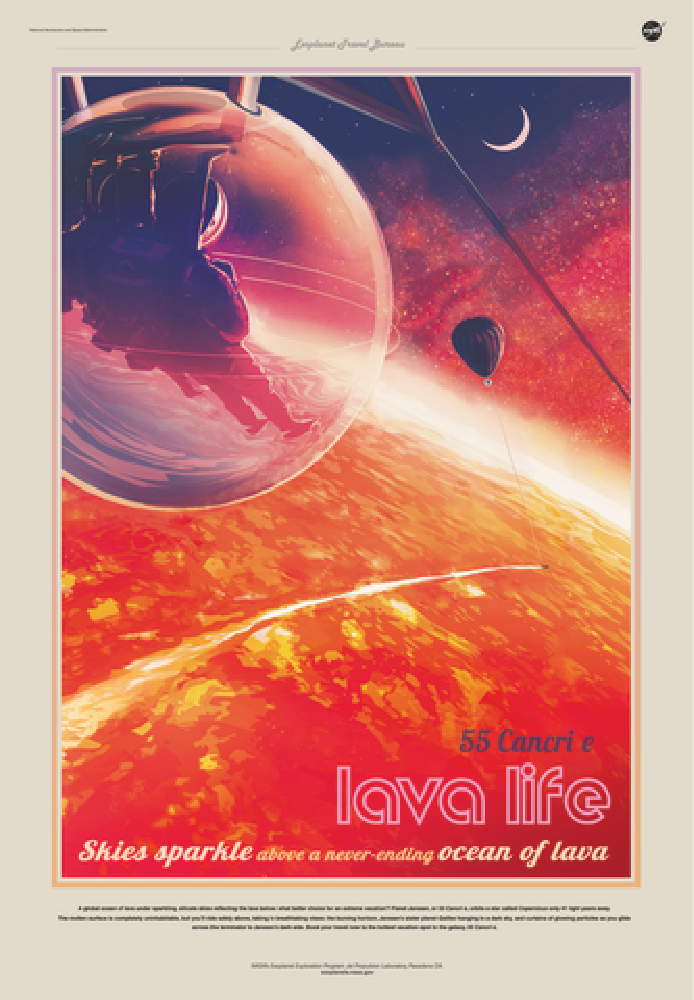
\includegraphics[height=2.2in]{images/55Cancri_e_FINAL_PRINT_1_30_small.pdf}}
\put(30, 60){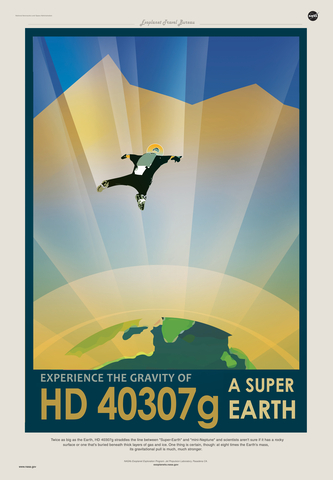
\includegraphics[height=2.2in]{images/HD_39x27_CMYK-1_small.jpg}}
\put(220, 55){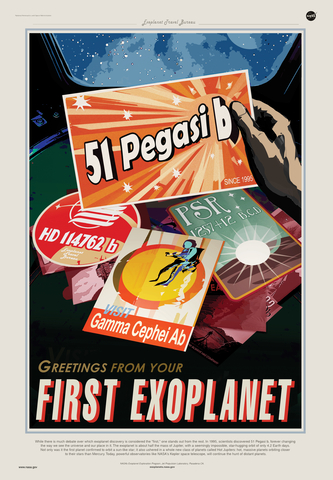
\includegraphics[height=2.2in]{images/First_exo_39x27_CMYK-1_small.jpg}}
\put(170, 60){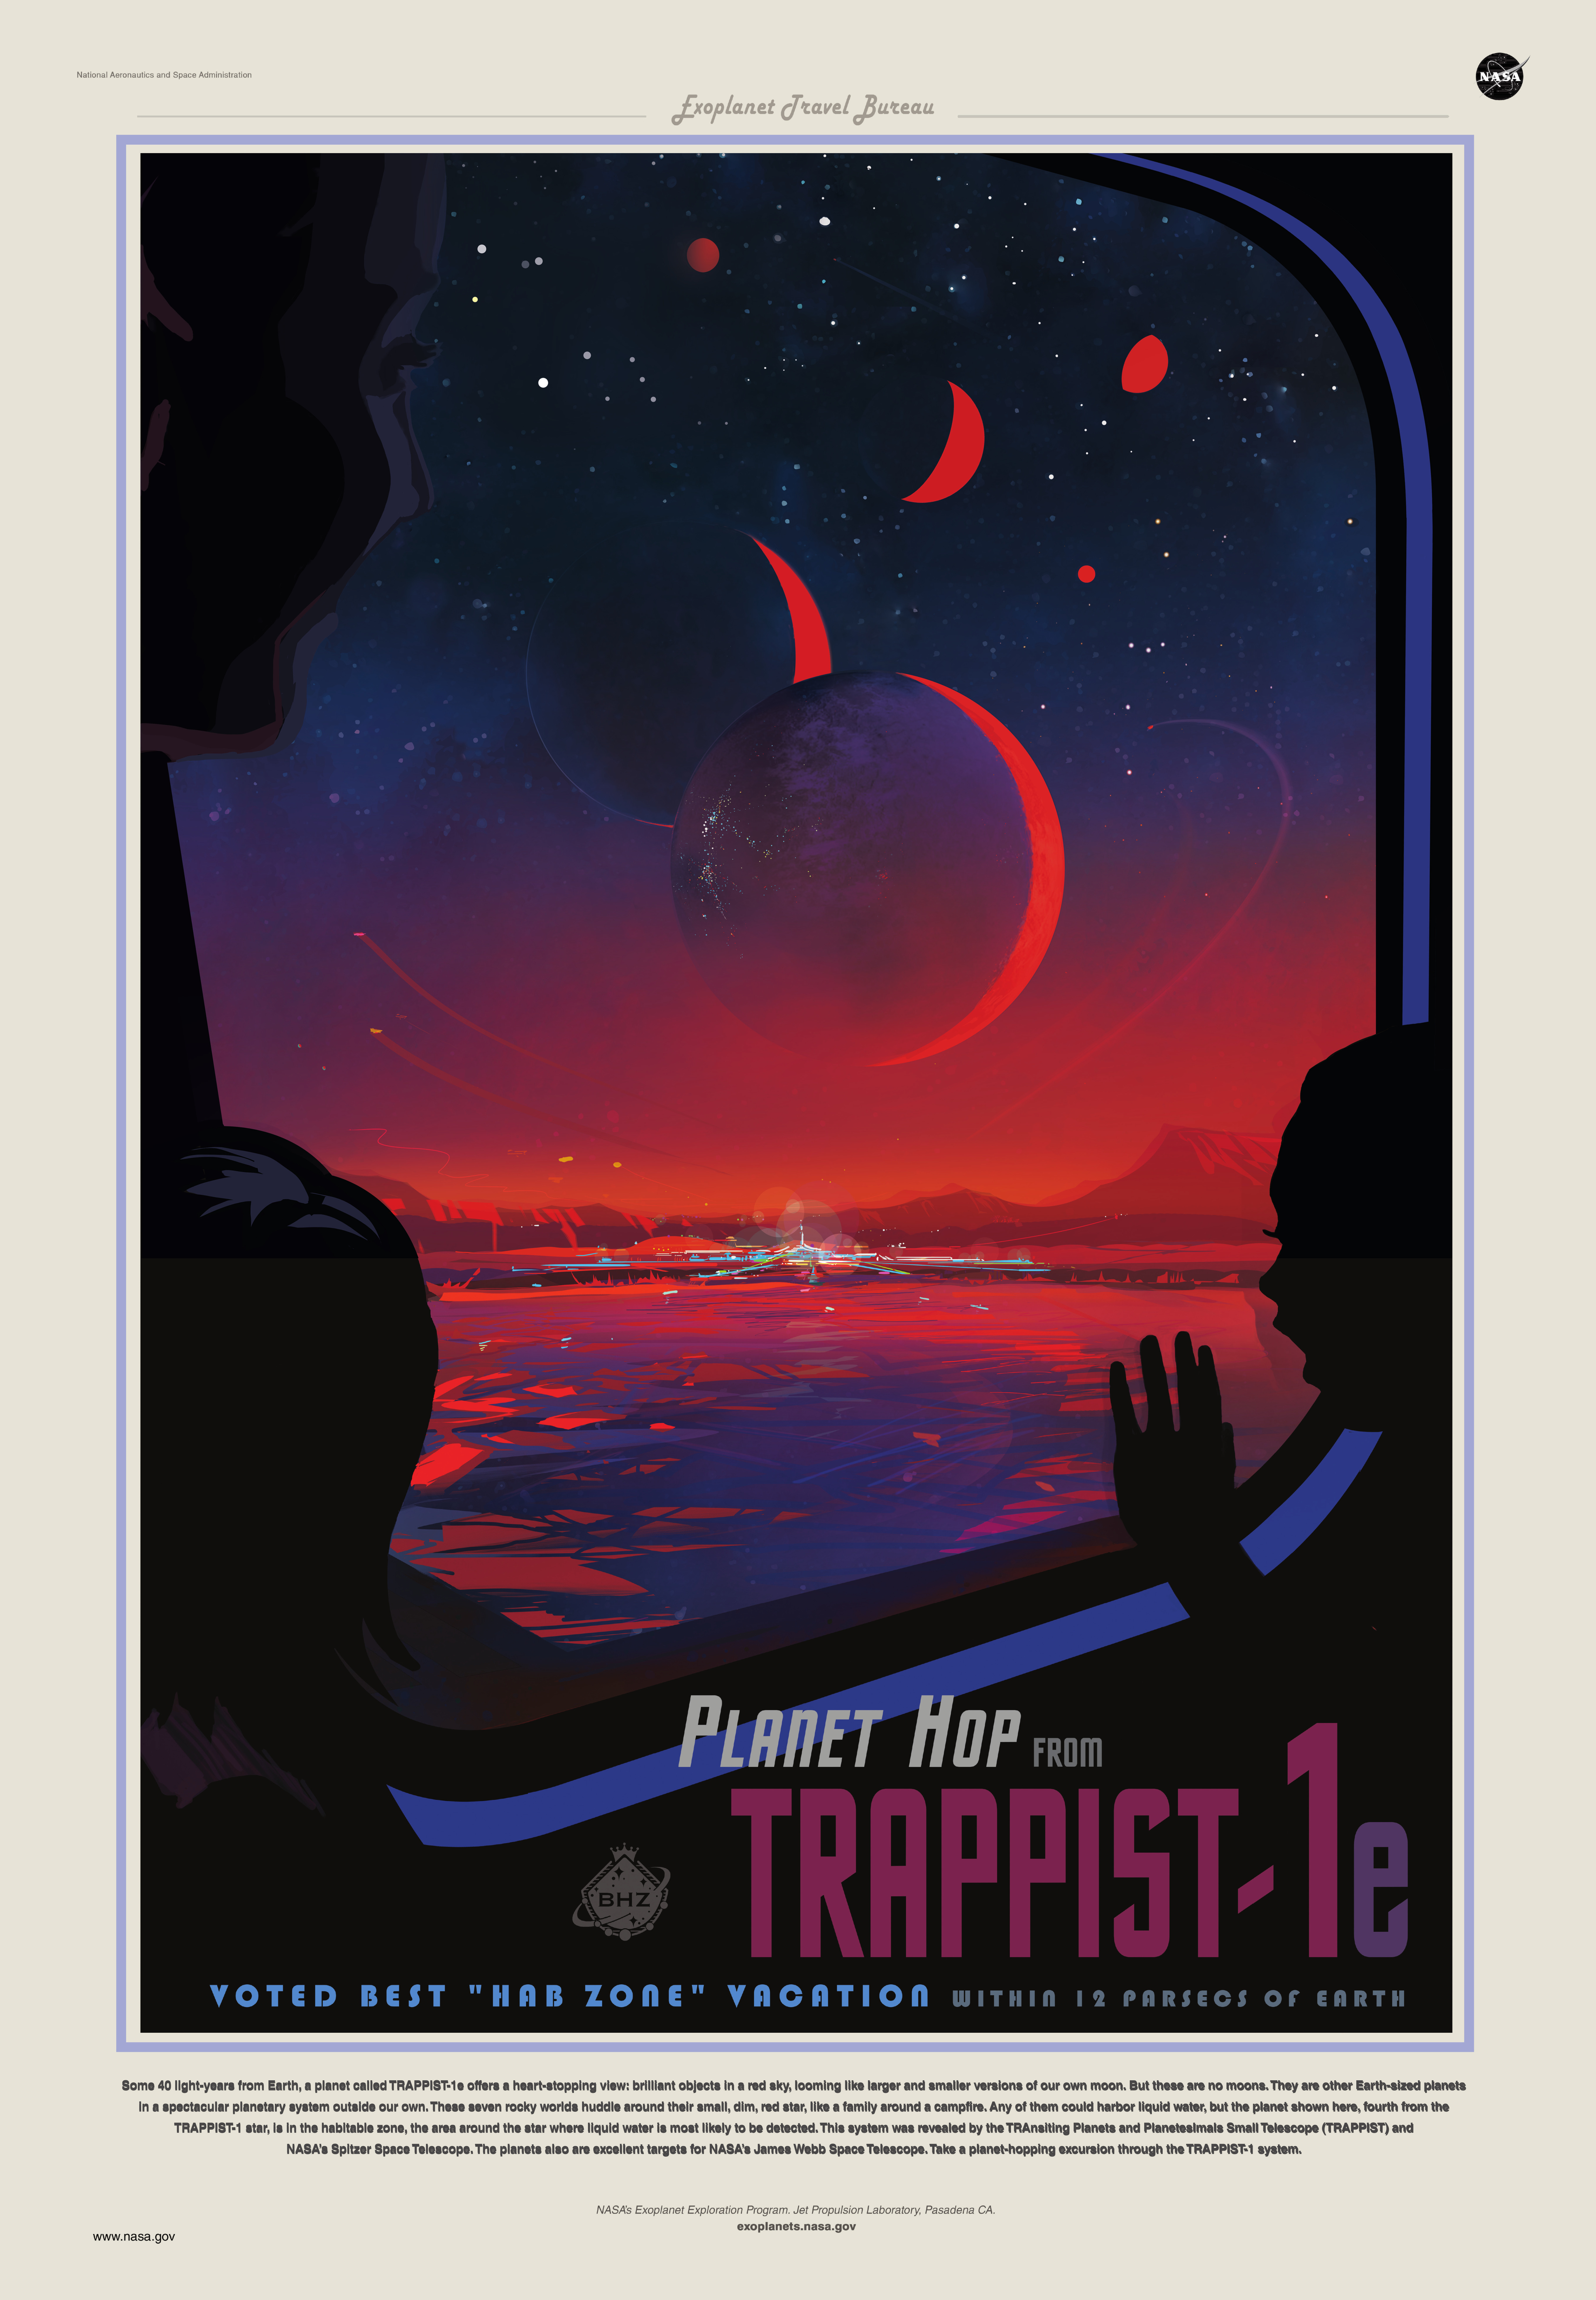
\includegraphics[height=2.2in]{images/TRAPPIST-1e_LEO_Const_CMYK_Print.jpg}}
\put(100, 65){\includegraphics[height=2.2in]{images/Rouge_39x27_CMYK-1.jpg}}
\put(107, 235){\begin{minipage}[t]{0.6 \linewidth}
{
Where is everybody?
}
\end{minipage}}
\end{picture}
\end{frame}


%\begin{frame}
%\frametitle{Omumguma}
%\end{frame}
%
%
% Drake eqn
% Fermi paradox
% Compute energy required to travel to alpha centari.
% Government interest, 
% Omumguma

%\section{Citations}
\begin{frame}
\begin{itemize}
    \item \scriptsize{https://www.scientificamerican.com/article/the-search-for-extraterre/}
    \item History Slides : \scriptsize{https://adsabs.harvard.edu/full/1981QJRAS..22..133T}
    \item \scriptsize{https://science.thewire.in/the-sciences/for-how-long-has-humankind-contemplated-aliens/}
    \item Movies and technical : \scriptsize{https://exoplanets.nasa.gov/}
    \item Farthest exoplanet : \scriptsize{https://en.wikipedia.org/wiki/SWEEPS-11}
    \item Direct imaging : \scriptsize{https://www.universetoday.com/140341/what-is-direct-imaging/}
    \item Optical Resolution Eqn: \scriptsize{https://en.wikipedia.org/wiki/Optical\_resolution}
    \item Kepler Space Telescope: \scriptsize{https://en.wikipedia.org/wiki/Kepler\_space\_telescope}
    \item TESS : \scriptsize{https://en.wikipedia.org/wiki/Transiting\_Exoplanet\_Survey\_Satellite}
    \item TESS : \scriptsize{https://en.wikipedia.org/wiki/James\_Webb\_Space\_Telescope}
    \item JWST : \scriptsize{https://en.wikipedia.org/wiki/James\_Webb\_Space\_Telescope}
    \item JWST field of view : \scriptsize{https://www.cosmos.esa.int/web/jwst-nirspec/home-old}
    \item JWST : \scriptsize{https://webb.nasa.gov/content/science/origins.html}
    \item SKA : \scriptsize{https://en.wikipedia.org/wiki/Square\_Kilometre\_Array}
    \item SKA and ETI : \scriptsize{https://arxiv.org/abs/1412.4867}
    \item Prevelance of Earth like planets : \scriptsize{https://www.pnas.org/content/110/48/19273}
\end{itemize}
\end{frame}


\begin{frame}
\begin{itemize}
    \item \scriptsize{Drake Equation : \scriptsize{https://www.seti.org/drake-equation-index}}
    \item Habitable rocky planets : \scriptsize{https://www.nasa.gov/feature/ames/kepler-occurrence-rate}
    \item Fraction of habitable planets : \scriptsize{https://www.nasa.gov/feature/ames/kepler-occurrence-rate}
    \item Fermi Paradox : \scriptsize{https://en.wikipedia.org/wiki/Fermi\_paradox}
    \item Estimate Age of Stars : \scriptsize{https://rechneronline.de/planets/lifespan-star.php}
    \item Nasa Exoplanet Archive : \scriptsize{https://exoplanetarchive.ipac.caltech.edu/docs/counts\_detail.html}
    \item Copernican Principle : \scriptsize{https://en.wikipedia.org/wiki/Copernican\_principle}
    % Unused links : 
    %% Fraction / Distribution of planets 
    %% https://www.pnas.org/content/111/35/12647
    %% https://iopscience.iop.org/article/10.3847/1538-3881/ab31ab/pdf
    %% Prevalence of Earth-size planets orbiting Sun-like stars : https://iopscience.iop.org/article/10.3847/1538-3881/ab31ab
    %% Nasa Earth-like planets Math worksheet : https://spacemath.gsfc.nasa.gov/news/7Page65.pdf
    %% Joint Mass-Radius-Period Distribution of Exoplanets : https://iopscience.iop.org/article/10.3847/1538-4357/ab6a92/pdf
    %% Exoplanet Demographics Beyond Kepler : https://exoplanets.nasa.gov/internal_resources/1937/
    %% Evolution of Exoplanet Size Distribution : https://iopscience.iop.org/article/10.3847/1538-3881/abf439/pdf
    %% Exoplanet Archive Data : https://exoplanetarchive.ipac.caltech.edu/cgi-bin/TblView/nph-tblView?app=ExoTbls&config=PS
    %% Outlining the Exoplanet Science Strategy : https://www.nap.edu/read/25187/chapter/5
    %% List of exoplanet extremes (wiki) : https://en.wikipedia.org/wiki/List_of_directly_imaged_exoplanets
\end{itemize}
\end{frame}

\begin{frame}
\frametitle{Images}
\begin{itemize}
    \item \chref{https://en.wikipedia.org/wiki/Plato\#/media/File:Plato\_Silanion\_Musei\_Capitolini\_MC1377.jpg}{Plato - Public Domain}
    \item \chref{https://en.wikipedia.org/wiki/Aristotle\#/media/File:Aristotle\_Altemps\_Inv8575.jpg}{Aristotle - Public Domain}
    \item \chref{https://en.wikipedia.org/wiki/Democritus\#/media/File:Democritus2.jpg}{Democritus - Public Domain}
    \item \chref{https://commons.wikimedia.org/wiki/File:Plutarch\_of\_Chaeronea-03\_(cropped).jpg}{Plutarch - CC BY-SA 4.0}
    \item \chref{https://www.imdb.com/title/tt0094574/mediaviewer/rm765168385}{Unsolved Mysteries - Fair Use}
    \item \chref{https://www.imdb.com/title/tt0083866/mediaviewer/rm1993282560/}{ET - Fair Use}
    \item \chref{https://www.amazon.com/Lost-Book-Enki-Prophecies-Extraterrestrial-ebook/dp/B004P1JEUW}{The Lost Book of Enky - Fair Use}
    \item \chref{https://newrepublic.com/article/126715/x-files-i-want-believe-posters-origin-story}{The X-Files - Fair Use}
    \item \chref{https://en.wikipedia.org/wiki/Thomas\_Aquinas\#/media/File:St-thomas-aquinas.jpg}{St. Thomas Aquinus - Public Domain }
    \item \chref{https://en.wikipedia.org/wiki/Albertus\_Magnus\#/media/File:AlbertusMagnus.jpg}{St. Albertus Magnus - Public Domain }
    \item \chref{https://en.wikipedia.org/wiki/Augustine\_of\_Hippo\#/media/File:Antonio\_Rodr\%C3\%ADguez\_-\_Saint\_Augustine\_-\_Google\_Art\_Project.jpg}{St. Augustine - Public Domain}
    \item \chref{https://en.wikipedia.org/wiki/Johannes\_Kepler\#/media/File:JKepler.jpg}{Johannes Kepler- Public Domain}
    \item \chref{https://en.wikipedia.org/wiki/Nicolaus\_Copernicus\#/media/File:Nikolaus\_Kopernikus.jpg}{Nicolaus Copernicus - Public Domain}
    \item \chref{https://en.wikipedia.org/wiki/Galileo\_Galilei\#/media/File:Justus\_Sustermans\_-\_Portrait\_of\_Galileo\_Galilei,\_1636.jpg}{Galileo Galilei - Public Domain}
\end{itemize}
\end{frame}


\begin{frame}
\frametitle{Images}
\begin{itemize}
    \item \chref{https://en.wikipedia.org/wiki/Arthur\_Eddington\#/media/File:Arthur\_Stanley\_Eddington.jpg}{Arthur Eddington - Public Domain}
    \item \chref{https://en.wikipedia.org/wiki/Percival\_Lowell\#/media/File:Percival\_Lowell\_1900s2.jpg}{Percival Lowell - Public Domain}
    \item \chref{https://en.wikipedia.org/wiki/Carl\_Sagan\#/media/File:Carl\_Sagan\_Planetary\_Society\_cropped.png}{Carl Sagan - Public Domain}
    \item \chref{https://www.eso.org/public/news/eso0842/}{Beta Pictoris b - Fair Use}
    \item \chref{https://www.eso.org/public/archives/releases/sciencepapers/eso0842/eso0842.pdf}{Beta Pictoris b - Fair Use}
    \item \chref{https://en.wikipedia.org/wiki/Kepler\_space\_telescope\#/media/File:Kepler\_Space\_Telescope\_spacecraft\_model\_2.png}{Kepler Space Telescope - Public Domain}
    \item \chref{https://en.wikipedia.org/wiki/Transiting\_Exoplanet\_Survey\_Satellite\#/media/File:TESS\_alone\_high\_res.jpg}{TESS - Public Domain}
    \item \chref{https://en.wikipedia.org/wiki/James\_Webb\_Space\_Telescope\#/media/File:JWST\_spacecraft\_model\_2.png}{JWST - Public Domain}
    \item \chref{https://webb.nasa.gov/content/science/origins.html}{Spectra - Public Domain}
    \item \chref{https://science.nasa.gov/science-pink/s3fs-public/atoms/files/3a.\%202018\%2009\_Exoplanet\%20Science\%20Strategy.pdf}{Period vs Mass - Public Domain}
    \item \chref{https://en.wikipedia.org/wiki/Square\_Kilometre\_Array\#/media/File:SKA\_overview.jpg}{SKA - CC-By-3.0 }
    \item \chref{https://www.nap.edu/read/25187/chapter/5\#55}{Period vs Mass - Fair Use}
    \item \chref{https://www.nasa.gov/sites/default/files/images/718509main\_lores.jpg}{Exoplanet Size - Fair Use}
    \item \chref{https://commons.wikimedia.org/w/index.php?curid=55463078}{HR 8799 by Jason Wang (Caltech)/Christian Marois (NRC Herzberg), - CC BY 3.0}
    \item \chref{https://commons.wikimedia.org/w/index.php?curid=436222}{Nicholas of Cusa - Public Domain}
    \item \chref{https://exoplanets.nasa.gov/alien-worlds/exoplanet-travel-bureau/}{Nasa Travel Posters - Public Domain}
    \item \chref{https://exoplanets.nasa.gov/search-for-life/habitable-zone/}{Habitable Zone - Fair Use}
\end{itemize}
\end{frame}
%%%  
%%%  
%%%  
\end{document}
